\documentclass[11pt]{amsart}

\usepackage[T1]{fontenc}
\usepackage{lmodern}
\usepackage{amssymb,amsmath}
\usepackage{booktabs,array}
\usepackage{graphicx}
\usepackage[dvipsnames]{xcolor}
\usepackage[margin=1.15in]{geometry}
\usepackage[colorlinks=true,linkcolor=blue!50!black,citecolor=blue!50!black,urlcolor=blue!50!black]{hyperref}

\newtheorem{theorem}{Theorem}[section]
\newtheorem{proposition}[theorem]{Proposition}
\newtheorem{lemma}[theorem]{Lemma}
\newtheorem{corollary}[theorem]{Corollary}
\theoremstyle{definition}
\newtheorem{definition}[theorem]{Definition}
\theoremstyle{remark}
\newtheorem{remark}[theorem]{Remark}

\numberwithin{equation}{section}
\numberwithin{table}{section}
\numberwithin{figure}{section}

\newcommand{\R}{\mathbb{R}}
\newcommand{\Z}{\mathbb{Z}}
\newcommand{\M}{\mathcal{M}}
\newcommand{\Rk}{\mathcal{R}}
\newcommand{\Sym}{\mathrm{Sym}}
\newcommand{\Min}{\operatorname{Min}}
\newcommand{\covol}{\operatorname{covol}}
\newcommand{\dist}{\operatorname{dist}}
\newcommand{\adj}{\operatorname{adj}}
\newcommand{\GL}{\mathrm{GL}}
\newcommand{\cand}{\mathcal{C}}
\newcommand{\one}{\mathbf{1}}
\newcommand{\T}{\mathsf{T}}
\hypersetup{pdftitle={Densest packings of two translates of a lattice in five dimensions},pdfauthor={Deep Bhattacharjee and Ushashi Bhattacharya}}
\providecommand{\doi}[1]{\href{https://doi.org/#1}{doi:\detokenize{#1}}}
\newcommand{\zenodoID}{10.5281/zenodo.23323366}
\newcommand{\preprintURL}{https://github.com/creelie/D5/blob/main/preprintAndreanovKallusTwoPeriodicPackingD5/AndreanovKallusTwoPeriodicPackingD5.pdf}

\raggedbottom
\begin{document}

\title[Packings of two lattice translates in five dimensions]{Densest packings of two translates\\ of a lattice in five dimensions}

\author{Deep Bhattacharjee}
\address{Formerly, Electro-Gravitational Space Propulsion Laboratory (EGSPL),\newline Bhubaneswar, Odisha 751030, India}
\email{itsdeep@live.com}
\email{d.bhattacharjee@erl-forschung.de}
\author{Ushashi Bhattacharya}
\address{Formerly, National Taiwan University, Taipei 106319, Taiwan}
\email{rai.bhattacharya.in@gmail.com}
\thanks{Corresponding author: Deep Bhattacharjee. ORCID iDs: Deep Bhattacharjee \href{https://orcid.org/0000-0003-0466-750X}{\mbox{0000-0003-0466-750X}}; Ushashi Bhattacharya \href{https://orcid.org/0009-0002-2254-3914}{\mbox{0009-0002-2254-3914}}.}

\subjclass[2020]{Primary 52C17; Secondary 11H31, 11H55}
\keywords{sphere packing, periodic packing, $D_5$ lattice, Ryshkov polyhedron, deep hole, Voronoi cell}

\begin{abstract}
We prove that no packing of unit balls in $\R^5$ whose centres form two translates of a lattice is denser than the $D_5$ lattice packing. Up to congruence exactly three such packings attain this density: $\sqrt2\,D_5$, a layered packing of Leech, and the packing with Szöllősi's kissing configuration.
\end{abstract}

\maketitle

\section{Introduction}

The root lattice $D_5=\{x\in\Z^5:x_1+\dots+x_5\in2\Z\}$~\cite[Ch.~4, \S7.1]{CS1999}, scaled by $\sqrt2$ so that its minimal distance is $2$, carries a packing of unit balls of density $\pi^2/(15\sqrt2)$. Korkine and Zolotarev proved that no lattice packing of balls in $\R^5$ is denser~\cite{KZ1877}. Whether $D_5$ is densest among all packings in $\R^5$ is open, and non-lattice packings of the same density exist: Leech constructed three~\cite{Leech1967}, Conway and Sloane placed them in a family of layered packings~\cite{CS1995}, and Cohn and Rajagopal~\cite{CR2026} found further examples after Szöllősi's discovery of a new kissing configuration of $40$ points~\cite{Szollosi2023}.

A periodic packing is a finite union of translates of one lattice. After lattices, the next case is two translates, $P=\Lambda\cup(\Lambda+b)$. Andreanov and Kallus~\cite{AK2020} extended Voronoi's algorithm for perfect forms~\cite{Voronoi1908} to such sets. In dimension $5$ their enumeration found that the maximal density is that of $D_5$, attained by five configurations, three of which represent $D_5$. Parts of their computation used floating-point arithmetic, and they present these results as numerical rather than rigorous~\cite[\S4]{AK2020}. Cohn and Rajagopal cite the bound as a theorem of~\cite{AK2020}~\cite[\S4.2]{CR2026}. We prove the bound together with the list of equality cases. The four-dimensional statement is proved in~\cite{Bha2026a}.

Throughout, $\Lambda_m$ and $b_m$ denote the lattices and vectors of Table~\ref{tab:five}, and $P_m=\Lambda_m\cup(\Lambda_m+b_m)$. Each $\Lambda_m$ has covolume $4$ and minimal norm $2$. Two pairs $(\Lambda,b)$ and $(\Lambda',b')$ are \emph{congruent} if an isometry of $\R^5$ maps $\Lambda$ onto $\Lambda'$ and $\Lambda+b$ onto $\Lambda'+b'$.

\begin{table}[t]
\centering
\small
\renewcommand{\arraystretch}{1.2}
\begin{tabular}{@{}c l c c c@{}}
\toprule
$m$ & $\Lambda_m$ & $b_m$ & $|\Min\Lambda_m|$ & $P_m$\\
\midrule
0 & $\{x\in\Z^5:x_1+x_2+x_3,\ x_4+x_5\in2\Z\}=D_3\oplus D_2$ & $e_1+e_4$ & 16 & $D_5$\\
1 & $A_4\oplus\Z\,\tfrac45\one$, \quad $A_4=\{x\in\Z^5:\sum x_i=0\}$ & $e_1+e_5$ & 20 & not a lattice\\
2 & $(D_4\times0)+\Z(h+2e_5)$, \quad $h=\tfrac12(e_1+e_2+e_3+e_4)$ & $e_1+e_5$ & 24 & not a lattice\\
3 & $\{x\in\Z^5:x_1+x_2+x_3+x_4,\ x_5\in2\Z\}=D_4\oplus2\Z$ & $e_1+e_5$ & 24 & $D_5$\\
4 & $\{x\in\Z^5:x_1+\dots+x_5\in4\Z\}$ & $e_1+e_2$ & 20 & $D_5$\\
\bottomrule
\end{tabular}
\caption{The five extremal configurations, at minimal distance $\sqrt2$. Here $\one=(1,1,1,1,1)$, $D_n=\{x\in\Z^n:\sum x_i\in2\Z\}$, and $|\Min\Lambda_m|$ is the number of vectors of norm $2$ in $\Lambda_m$.}
\label{tab:five}
\end{table}

\begin{theorem}\label{thm:main}
Let $\Lambda\subset\R^5$ be a lattice and $b\in\R^5\setminus\Lambda$ such that $|x-y|\ge2$ for all distinct $x,y\in P=\Lambda\cup(\Lambda+b)$. Then $\covol(\Lambda)\ge16\sqrt2$. Equality holds if and only if $(\Lambda,b)$ is congruent to $(\sqrt2\,\Lambda_m,\sqrt2\,b_m)$ for some $m\in\{0,\dots,4\}$, and these five pairs are pairwise not congruent. Equivalently, the packing of unit balls centred at $P$ has density at most $\pi^2/(15\sqrt2)$, and equality holds exactly when $P$ is congruent to $\sqrt2\,D_5$, $\sqrt2\,P_1$ or $\sqrt2\,P_2$.
\end{theorem}

The sets $P_0$, $P_3$, $P_4$ are $D_5$ split into two cosets of a sublattice of index two; the $31$ such sublattices form three orbits under the symmetries of $D_5$, and $\Lambda_0,\Lambda_3,\Lambda_4$ represent them (Remark~\ref{rem:identify}). The set $\sqrt2\,P_1$ is the uniform packing with Szöllősi's kissing configuration $Q_5$, found by Andreanov and Kallus and described by Cohn and Rajagopal~\cite[Table~4.2]{CR2026}. The set $\sqrt2\,P_2$ is the layered packing of Leech whose kissing configuration is $L_5$~\cite{Leech1967,CR2026}. The three sets are pairwise not congruent.

A lattice $L$ is the union of two cosets of any sublattice $\Lambda$ of index two, with $\covol(L)=\frac12\covol(\Lambda)$. So Theorem~\ref{thm:main} contains the five-dimensional case of the theorem of Korkine and Zolotarev: a lattice in $\R^5$ with minimal distance $2$ has covolume at least $8\sqrt2$, with equality only for $\sqrt2\,D_5$. It also bounds the Voronoi cells.

\begin{corollary}\label{cor:cells}
Let $P\subset\R^5$ be a lattice, or a union of two translates of a lattice, such that distinct points of $P$ are at distance at least $2$. Every Voronoi cell of $P$ has volume at least $8\sqrt2$, the volume of the Voronoi cell of $\sqrt2\,D_5$. Equality holds if and only if $P$ is congruent to $\sqrt2\,D_5$, $\sqrt2\,P_1$ or $\sqrt2\,P_2$.
\end{corollary}

\begin{figure}[t]
\centering
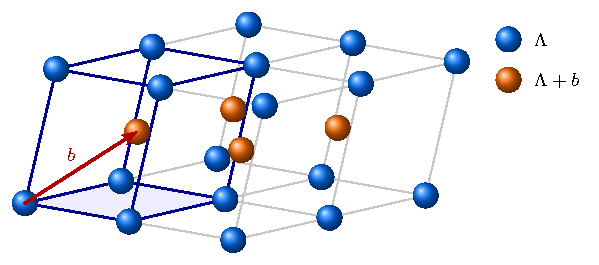
\includegraphics[width=0.8\textwidth]{figures/translates}
\caption{Two translates of a lattice, drawn in three dimensions: the points of $\Lambda$ and of $\Lambda+b$, with a cell spanned by a basis of $\Lambda$. Such a set is described by the Gram matrix of the basis together with $b$. In five dimensions the densest packings of unit balls centred at such sets are $\sqrt2\,D_5$, $\sqrt2\,P_1$ and $\sqrt2\,P_2$ (Theorem~\ref{thm:main}).}
\label{fig:translates}
\end{figure}

\subsection*{Method}
A pair $(\Lambda,b)$ is encoded by the $6\times6$ Gram matrix $J$ of a basis of $\Lambda$ together with $b$. The packing condition becomes infinitely many linear inequalities $J[k]\ge4$, which cut out a locally finite polyhedron $\Rk$ in the $21$-dimensional space of symmetric matrices (Section~\ref{sec:polyhedron}). Packings are the points of $\Rk$ with $\det J=0$, and the quantity to minimise is $\det Q$, where $Q$ is the upper left $5\times5$ block of $J$. Proposition~\ref{prop:descent} moves every packing, without increasing $\det Q$, to a vertex of $\Rk$ or to an interior point of an edge. The argument uses only the concavity of $\log\det Q$ and of the Schur complement of $Q$ in $J$.

Up to the integral symmetries of the problem, $\Rk$ has $34$ vertices and $480$ edges at them (Proposition~\ref{prop:computation}). This finite statement is computed in exact arithmetic and recorded in a certificate. Four independent implementations check the certificate, four independent enumerations recompute the extreme rays of the vertex cones, and a proof in Lean~4 checks in the kernel the minimal vectors and determinants of every vertex and the statements of the certificate on every listed edge (Appendix~\ref{app:verification} states exactly what is formalized). The $25$ unbounded edges are explicit (Table~\ref{tab:unbounded}). In dimension four every vertex other than the optimum has $\det J>0$; in dimension five two vertices have $\det J<0$, and the bounded edges at them carry packings (Remark~\ref{rem:bounded}).

The equality case is proved by hand in Section~\ref{sec:equality}. A deep hole of a lattice is surrounded by lattice points that span the space affinely (Lemma~\ref{lem:deephole}). Perturbing along the directions of $\Rk$ at an extremal configuration then shows that it is a vertex or an interior point of an edge of $\Rk$, so it appears in the finite list (Proposition~\ref{prop:equality}). Section~\ref{sec:five} identifies the five configurations.

\section{Two-periodic sets and the polyhedron \texorpdfstring{$\Rk$}{R}}\label{sec:polyhedron}

\subsection{Notation}
$\Sym_n$ is the space of real symmetric $n\times n$ matrices, with any fixed norm $\|\cdot\|$. For $J\in\Sym_6$ and $x\in\R^6$ we write $J[x]=x^\T Jx$, and
\[
J=\begin{pmatrix}Q&r\\ r^\T&s\end{pmatrix},\qquad Q=Q(J)\in\Sym_5,\ r\in\R^5,\ s\in\R .
\]
Let $\M=\Z^5\times\{-1,0,1\}\subset\Z^6$ and $\M^*=\M\setminus\{0\}$. Elements of $\M$ are written $k=(n,l)$ with $n\in\Z^5$ and $l\in\{-1,0,1\}$. Define
\[
\Rk=\{J\in\Sym_6:\ J[k]\ge4\ \text{for all }k\in\M^*\}.
\]
$\Rk$ is closed and convex. For $J\in\Rk$ let
\begin{gather*}
\Min(J)=\{k\in\M^*:J[k]=4\},\qquad C_J=\{X\in\Sym_6: X[k]\ge0\ \text{for all } k\in\Min(J)\},\\
L_J=C_J\cap(-C_J)=\{X\in\Sym_6:X[k]=0\ \text{for all }k\in\Min(J)\},
\end{gather*}
and $d(J)=\dim L_J$. Since $k$ and $-k$ give the same condition, we list one vector of each pair $\pm k$ when counting $\Min(J)$.

Let $\Lambda\subset\R^5$ be a lattice with basis $a=(a_1,\dots,a_5)$ and let $b\in\R^5$. The Gram matrix of $(a_1,\dots,a_5,b)$ is denoted $J(a,b)$, so that
\begin{equation}\label{eq:J}
J(a,b)[(n,l)]=\Bigl|\sum_{i=1}^5 n_ia_i+lb\Bigr|^2 .
\end{equation}

\begin{lemma}\label{lem:packing}
Let $b\notin\Lambda$. The distinct points of $\Lambda\cup(\Lambda+b)$ are at distance at least $2$ if and only if $J(a,b)\in\Rk$.
\end{lemma}

\begin{proof}
Since $\Lambda$ and $\Lambda+b$ are disjoint, the differences of distinct points are the vectors of $(\Lambda\setminus0)\cup(\Lambda+b)\cup(\Lambda-b)$, that is, the vectors $\sum n_ia_i+lb$ with $(n,l)\in\M^*$. Apply~\eqref{eq:J}.
\end{proof}

\begin{lemma}\label{lem:pd}
For $J\in\Rk$ the block $Q(J)$ is positive definite.
\end{lemma}

\begin{proof}
We have $Q[n]=J[(n,0)]\ge4$ for $n\in\Z^5\setminus0$. If $Q[x]<0$ for some $x\in\R^5$, the open cone $\{Q<0\}$ contains a rational point and hence an integral point $n\ne0$ with $Q[n]<0$, a contradiction. So $Q$ is positive semidefinite. Suppose $Qv=0$ with $\max_i|v_i|=1$. By Dirichlet's theorem on simultaneous approximation, for every integer $N\ge1$ there are an integer $1\le m\le N^5$ and $n\in\Z^5$ with $\max_i|mv_i-n_i|\le1/N$. Then $n\ne0$ because $\max_i|mv_i|=m\ge1>1/N$, and $Q[n]=Q[n-mv]\le25\|Q\|_{\infty}/N^2$, where $\|Q\|_\infty$ is the largest absolute value of an entry. For large $N$ this is less than $4$, a contradiction. Hence $Q$ is positive definite.
\end{proof}

Let $\Sym_6^+=\{J\in\Sym_6:Q(J)\text{ positive definite}\}$, an open convex set containing $\Rk$. For $J\in\Sym_6^+$ put
\[
q(J)=Q^{-1}r,\qquad \sigma(J)=s-r^\T Q^{-1}r .
\]

\begin{lemma}\label{lem:sigma}
Let $J\in\Sym_6^+$.
\begin{enumerate}
\item $J[(x,l)]=Q[x+l\,q(J)]+l^2\sigma(J)$ for $x\in\R^5$ and $l\in\R$.
\item $\sigma(J)=\min_{x\in\R^5}J[(x,1)]$, attained at $x=-q(J)$. In particular $\sigma(J')\le J'[u]$ for every $J'\in\Sym_6^+$ and every $u\in\R^5\times\{1\}$, and $\sigma$ is concave on $\Sym_6^+$.
\item $\det J=\det Q\cdot\sigma(J)$.
\end{enumerate}
\end{lemma}

\begin{proof}
(1) is completing the square, (2) follows from (1) because $Q$ is positive definite, and a minimum of affine functions of $J$ is concave. (3) is the Schur complement formula.
\end{proof}

\begin{lemma}\label{lem:rank5}
Let $J\in\Rk$.
\begin{enumerate}
\item $\sigma(J)=0$ if and only if $J=J(a,b)$ for a basis $a$ of a lattice $\Lambda\subset\R^5$ and a vector $b\notin\Lambda$ such that the distinct points of $\Lambda\cup(\Lambda+b)$ are at distance at least $2$. In that case $\det Q(J)=\covol(\Lambda)^2$.
\item If $\sigma(J)<0$, then $J+|\sigma(J)|\,e_6e_6^\T\in\Rk$, its $Q$-block is $Q(J)$, and its $\sigma$ is $0$.
\end{enumerate}
\end{lemma}

\begin{proof}
(1) If $\sigma(J)=0$, then $J$ is positive semidefinite of rank $5$ by Lemma~\ref{lem:sigma}(1), (3) and Lemma~\ref{lem:pd}, hence the Gram matrix of six vectors $a_1,\dots,a_5,b$ of $\R^5$, and $a_1,\dots,a_5$ are linearly independent because $Q$ is positive definite. If $b$ were $\sum n_ia_i$, then $J[(-n,1)]=0<4$. Lemma~\ref{lem:packing} gives the packing property. Conversely $J(a,b)$ is a Gram matrix of six vectors in $\R^5$, so $\det J(a,b)=0$ and $\sigma=0$ by Lemma~\ref{lem:sigma}(3). Finally $\det Q=\det(a_i\cdot a_j)=\covol(\Lambda)^2$.
(2) Adding $|\sigma|e_6e_6^\T$ changes $J[(n,l)]$ by $l^2|\sigma|\ge0$, leaves $Q$ and $r$ unchanged and raises $s$, hence $\sigma$, by $|\sigma|$.
\end{proof}

\begin{lemma}\label{lem:minkowski}
For $J\in\Rk$, $\det Q(J)\ge64\pi^4/225$.
\end{lemma}

\begin{proof}
$Q$ is the Gram matrix of a lattice $\Lambda$ with no nonzero vector of length less than $2$. The open ball of radius $2$ in $\R^5$ has volume $2^5\cdot8\pi^2/15$. By Minkowski's convex body theorem~\cite[Ch.~III]{Cassels1959} it contains a nonzero point of $\Lambda$ if its volume exceeds $2^5\covol(\Lambda)$. Hence $\covol(\Lambda)\ge8\pi^2/15$.
\end{proof}

\subsection{Local structure}

\begin{lemma}\label{lem:local}
\begin{enumerate}
\item For every compact set $K\subset\Sym_6^+$ the set $\M_K=\{k\in\M^*: J[k]\le5\text{ for some }J\in K\}$ is finite.
\item For every $J\in\Rk$ there is $\varepsilon>0$ such that for all $X\in\Sym_6$ with $\|X\|\le\varepsilon$ we have $J+X\in\Rk$ if and only if $X\in C_J$.
\item For every $J\in\Rk$, $\Min(J)$ is finite and $\Rk\subseteq J+C_J$.
\end{enumerate}
\end{lemma}

\begin{proof}
(1) On $K$ the smallest eigenvalue of $Q$ is at least some $\mu>0$, and $|q(J)|\le\rho$, $|\sigma(J)|\le\rho$ for some $\rho$, by continuity. For $k=(n,l)\in\M^*$ and $J\in K$, Lemma~\ref{lem:sigma}(1) gives $J[k]\ge\mu|n+lq(J)|^2-\rho$. If $|n|>\rho+\sqrt{(5+\rho)/\mu}$, then $|n+lq(J)|\ge|n|-\rho$ and $J[k]>5$.
(2) Choose $\varepsilon_0>0$ such that the closed ball $K=\bar B(J,\varepsilon_0)$ lies in $\Sym_6^+$. The finitely many $k\in\M_K\setminus\Min(J)$ have $J[k]>4$, so there is $\varepsilon\le\varepsilon_0$ with $(J+X)[k]>4$ for all of them whenever $\|X\|\le\varepsilon$. For such $X$, the vectors $k\notin\M_K$ satisfy $(J+X)[k]>5$, so $J+X\in\Rk$ if and only if $(J+X)[k]=4+X[k]\ge4$ for all $k\in\Min(J)$.
(3) $\Min(J)\subseteq\M_{\{J\}}$ is finite. If $J'\in\Rk$, then $J+\lambda(J'-J)\in\Rk$ for $\lambda\in[0,1]$, and by (2) $\lambda(J'-J)\in C_J$ for small $\lambda>0$; $C_J$ is a cone.
\end{proof}

\begin{lemma}\label{lem:nolines}
$\Rk$ contains no line.
\end{lemma}

\begin{proof}
If $J+\tau X\in\Rk$ for all $\tau\in\R$, then $X[k]=0$ for every $k\in\M^*$. The matrices $kk^\T$ for $k=e_i$ $(1\le i\le6)$ and $k=e_i+e_j$ $(1\le i<j\le6)$, all in $\M^*$, span $\Sym_6$, so $X=0$.
\end{proof}

\begin{definition}
A \emph{vertex} of $\Rk$ is a point $J\in\Rk$ with $d(J)=0$. Then $C_J$ is a pointed polyhedral cone, defined by the finitely many inequalities $X[k]\ge0$, $k\in\Min(J)$, whose linear forms span the $21$-dimensional dual of $\Sym_6$. An \emph{extreme ray} of $C_J$ is a ray $\R_{\ge0}Y$, $Y\ne0$, with $Y\in C_J$ such that the forms $X\mapsto X[k]$ for the $k\in\Min(J)$ with $Y[k]=0$ span a $20$-dimensional space. For an extreme ray $Y$ put
\[
t^*(J,Y)=\sup\{t\ge0:J+tY\in\Rk\}\in(0,\infty],
\]
which is positive by Lemma~\ref{lem:local}(2). The set $\{J+tY:0\le t\le t^*\}$ (with $t<\infty$) is the \emph{edge} of $\Rk$ at $J$ in direction $Y$; it is \emph{bounded} if $t^*<\infty$.
\end{definition}

We use two standard facts on polyhedral cones~\cite[Lecture~1]{Ziegler1995}: a pointed polyhedral cone has finitely many extreme rays and is their conical hull, and a nonzero vector of the cone spans an extreme ray exactly when the inequalities it satisfies with equality have rank one less than the dimension.

\begin{lemma}\label{lem:edges}
Let $J$ be a vertex and $Y$ an extreme ray of $C_J$, and let $Z=\{k\in\Min(J):Y[k]=0\}$.
\begin{enumerate}
\item $\{t\ge0:J+tY\in\Rk\}$ is the interval $[0,t^*]$, or $[0,\infty)$ if $t^*=\infty$. If $t^*<\infty$, then $J+t^*Y$ is a vertex.
\item For $0<t<t^*$ we have $\Min(J+tY)=Z$ and $d(J+tY)=1$.
\item Every $J'\in\Rk$ with $d(J')=1$ lies on an edge: $J'=J_v+tY'$ for a vertex $J_v$, an extreme ray $Y'$ of $C_{J_v}$, and $0<t<t^*(J_v,Y')$.
\end{enumerate}
\end{lemma}

\begin{proof}
(1) The set is convex and closed. Let $J_1=J+t^*Y$ with $t^*<\infty$. Every $k\in Z$ has $J_1[k]=4$, so $Z\subseteq\Min(J_1)$. Since $J_1+\eta Y\notin\Rk$ for $\eta>0$, Lemma~\ref{lem:local}(2) gives $Y\notin C_{J_1}$, so some $k_1\in\Min(J_1)$ has $Y[k_1]<0$. The forms of $Z$ vanish on $Y$ and span a $20$-dimensional space, and the form of $k_1$ does not vanish on $Y$; together they have rank $21$, so $L_{J_1}=0$.
(2) For $k\in\M^*$ the function $\tau\mapsto(J+\tau Y)[k]$ is affine and at least $4$ on $[0,t]$ and slightly beyond $t$. If it equals $4$ at $t$, it is constant, so $J[k]=4$ and $Y[k]=0$. Hence $\Min(J+tY)=Z$, and $L_{J+tY}$, cut out by the forms of $Z$ of rank $20$, has dimension $1$.
(3) Let $L_{J'}=\R X_0$. The set $I_0=\{\tau:J'+\tau X_0\in\Rk\}$ is a closed interval which contains a neighbourhood of $0$ by Lemma~\ref{lem:local}(2) and is not $\R$ by Lemma~\ref{lem:nolines}. Let $\tau_e$ be a finite end point, $J_v=J'+\tau_eX_0$ and $Y'=-\operatorname{sgn}(\tau_e)X_0$. Since $X_0[k]=0$ for $k\in\Min(J')$, we have $\Min(J')\subseteq\Min(J_v)$ and $L_{J_v}\subseteq L_{J'}$. If $X_0\in L_{J_v}$, then $J_v\pm\eta X_0\in\Rk$ for small $\eta$ by Lemma~\ref{lem:local}(2), contradicting the choice of $\tau_e$; so $d(J_v)=0$. The segment from $J_v$ to $J'$ lies in $\Rk$, so $Y'\in C_{J_v}$ by Lemma~\ref{lem:local}(2), and $Y'$ vanishes on $\Min(J')$, which has rank $20$; so $Y'$ spans an extreme ray of $C_{J_v}$, and $J'=J_v+|\tau_e|Y'$. Finally $|\tau_e|<t^*(J_v,Y')$, since otherwise $J'$ would be a vertex by (1).
\end{proof}

\subsection{Symmetries}\label{ssec:symmetries}
Let $\Gamma$ be the group of matrices
\[
T=\begin{pmatrix}U&v\\0&\varepsilon\end{pmatrix},\qquad U\in\GL_5(\Z),\ v\in\Z^5,\ \varepsilon\in\{1,-1\}.
\]
Then $T(n,l)=(Un+lv,\varepsilon l)$, so $T$ maps $\M$ bijectively onto itself, and $J\mapsto T^\T JT$ maps $\Rk$ bijectively onto itself with $(T^\T JT)[k]=J[Tk]$. Consequently $\Min(T^\T JT)=T^{-1}\Min(J)$, $X\mapsto T^\T XT$ maps $C_J$ onto $C_{T^\T JT}$, and vertices, extreme rays, edges and the values $t^*$ correspond. Moreover $Q(T^\T JT)=U^\T QU$, so $\det Q$, $\det J$ and $\sigma=\det J/\det Q$ are $\Gamma$-invariant. We call $J,J'$ \emph{equivalent} if $J'=T^\T JT$ for some $T\in\Gamma$, and write $\Gamma_J$ for the stabiliser of $J$.

\begin{lemma}\label{lem:congruent}
Let $a$, $a'$ be bases of lattices $\Lambda,\Lambda'\subset\R^5$ and $b,b'\in\R^5$. Then $J(a,b)$ and $J(a',b')$ are equivalent if and only if $(\Lambda,b)$ and $(\Lambda',b')$ are congruent.
\end{lemma}

\begin{proof}
Suppose $J(a',b')=T^\T J(a,b)T$ with $T$ as above. The vectors $(a',b')$ and $(aU,\varepsilon b+\sum v_ia_i)$ have the same Gram matrix, and $a'$ spans $\R^5$, so a linear isometry $\psi$ maps $a'$ to $aU$ and $b'$ to $\varepsilon b+\sum v_ia_i$. Then $\psi(\Lambda')=\Lambda$ and $\psi(\Lambda'+b')=\Lambda+\varepsilon b$. If $\varepsilon=-1$, replace $\psi$ by $-\psi$, which maps $\Lambda'$ onto $\Lambda$ and $\Lambda'+b'$ onto $\Lambda+b$. Conversely, let an isometry $f$ map $\Lambda'$ onto $\Lambda$ and $\Lambda'+b'$ onto $\Lambda+b$. Then $f(0)\in\Lambda$, and $\psi=f-f(0)$ is a linear isometry with $\psi(\Lambda')=\Lambda$ and $\psi(\Lambda'+b')=\Lambda+b$. So $\psi(a')=aU$ with $U\in\GL_5(\Z)$ and $\psi(b')=b+\sum v_ia_i$ with $v\in\Z^5$, and $J(a',b')=T^\T J(a,b)T$ with $\varepsilon=1$.
\end{proof}

\subsection{Reaching all vertices}

\begin{proposition}\label{prop:connected}
Let $v$ and $w$ be vertices of $\Rk$. There are vertices $v=v_0,v_1,\dots,v_m=w$ such that $v_{s+1}=v_s+t^*Y_s$ for an extreme ray $Y_s$ of $C_{v_s}$ with $t^*(v_s,Y_s)<\infty$.
\end{proposition}

\begin{proof}
Let $\ell(X)=\sum_{k\in\Min(w)}X[k]$. Then $\ell\ge0$ on $C_w$, and $\ell(X)=0$ for $X\in C_w$ only if $X\in L_w=0$. By compactness of $\{X\in C_w:\|X\|=1\}$ there is $\delta>0$ with $\ell(X)\ge\delta\|X\|$ on $C_w$. By Lemma~\ref{lem:local}(3), $\Rk\subseteq w+C_w$, so $\ell(J)>\ell(w)$ for $J\in\Rk\setminus\{w\}$, and for every $c$ the set $S_c=\{J\in\Rk:\ell(J)\le c\}$ is compact. A vertex $J$ is the unique solution of the linear equations $J[k]=4$, $k\in\Min(J)$, and the vertices in $S_c$ have $\Min(J)\subseteq\M_{S_c}$, a finite set by Lemma~\ref{lem:local}(1). So $S_c$ contains finitely many vertices.

Let $u$ be a vertex with $u\ne w$. If $\ell(Y)\ge0$ for every extreme ray of $C_u$, then $\ell\ge0$ on $C_u$, and $\Rk\subseteq u+C_u$ gives $\ell(w)\ge\ell(u)$, which is false. So some extreme ray $Y$ of $C_u$ has $\ell(Y)<0$. Along $u+tY$ the value of $\ell$ decreases, and $S_{\ell(u)}$ is compact, so $t^*(u,Y)<\infty$, and $u'=u+t^*Y$ is a vertex (Lemma~\ref{lem:edges}) with $\ell(u')<\ell(u)$. Starting from $u=v$ and repeating, we obtain a sequence of vertices in $S_{\ell(v)}$ along which $\ell$ strictly decreases. It is finite, and it can only stop at $w$.
\end{proof}

\begin{corollary}\label{cor:closure}
Let $J_0,\dots,J_N$ be vertices of $\Rk$ such that for every $i$ and every extreme ray $Y$ of $C_{J_i}$ with $t^*(J_i,Y)<\infty$ the vertex $J_i+t^*Y$ is equivalent to some $J_j$. Then every vertex of $\Rk$ is equivalent to some $J_j$, and every edge of $\Rk$ is equivalent to an edge at some $J_j$.
\end{corollary}

\begin{proof}
Let $w$ be a vertex and take the path $J_0=v_0,\dots,v_m=w$ of Proposition~\ref{prop:connected}. If $v_s=T^\T J_iT$, then $Y'=T^{-\T}Y_sT^{-1}$ is an extreme ray of $C_{J_i}$ with the same $t^*$, and $v_{s+1}=T^\T(J_i+t^*Y')T$, which is equivalent to some $J_j$ by hypothesis. By induction $w$ is equivalent to some $J_j$. An edge at a vertex $w=T^\T J_jT$ in direction $Y$ is the image under $T$ of the edge at $J_j$ in direction $T^{-\T}YT^{-1}$.
\end{proof}

\section{Reduction to vertices and edges}\label{sec:reduction}

\begin{lemma}\label{lem:logdet}
Let $Q$ be positive definite and $H\in\Sym_5$, $H\ne0$. On the open interval of $\tau$ where $Q+\tau H$ is positive definite, $\psi(\tau)=\log\det(Q+\tau H)$ is strictly concave.
\end{lemma}

\begin{proof}
With $Q_\tau=Q+\tau H$ we have $\psi'(\tau)=\operatorname{tr}(Q_\tau^{-1}H)$ and $\psi''(\tau)=-\operatorname{tr}\bigl((Q_\tau^{-1/2}HQ_\tau^{-1/2})^2\bigr)<0$, because $Q_\tau^{-1/2}HQ_\tau^{-1/2}$ is a nonzero symmetric matrix.
\end{proof}

Let
\[
S=\{J\in\Rk:\sigma(J)\le0\},\qquad
\cand=\{J\in S: d(J)=0\}\ \cup\ \{J\in\Rk: d(J)=1,\ \sigma(J)=0\}.
\]
So $\cand$ consists of the vertices with $\det J\le0$ and of the points with $\det J=0$ in the relative interiors of edges (Lemma~\ref{lem:edges}). By Lemma~\ref{lem:rank5}, the infimum of $\det Q$ over $S$ equals the infimum of $\covol(\Lambda)^2$ over the pairs of Theorem~\ref{thm:main}.

\begin{proposition}\label{prop:descent}
For every $J\in S$ there is $J'\in\cand$ with $\det Q(J')\le\det Q(J)$.
\end{proposition}

\begin{proof}
Write $f(J)=\log\det Q(J)$ and $\pi(J)=2d(J)+[\sigma(J)<0]$, where $[\cdot]$ is $1$ if the condition holds and $0$ otherwise. We show: if $J\in S\setminus\cand$, there is $J_1\in S$ with $f(J_1)\le f(J)$ and $\pi(J_1)<\pi(J)$. Induction on $\pi$ then proves the proposition.

Let $J\in S\setminus\cand$. Then either (a) $\sigma(J)<0$ and $d(J)\ge1$, or (b) $\sigma(J)=0$ and $d(J)\ge2$. In case (a) choose any $X\in L_J\setminus0$. In case (b) let $u=(-q(J),1)\in\R^6$, so that $J[u]=\sigma(J)=0$ by Lemma~\ref{lem:sigma}(2), and choose $X\in L_J\setminus0$ with $X[u]=0$, which exists because $\dim L_J\ge2$. Put $J(\tau)=J+\tau X$ and
\[
I_0=\{\tau\in\R:J(\tau)\in\Rk\}.
\]
$I_0$ is a closed interval, it contains a neighbourhood of $0$ by Lemma~\ref{lem:local}(2) because $\pm X\in C_J$, and $I_0\ne\R$ by Lemma~\ref{lem:nolines}. Since $X[k]=0$ for $k\in\Min(J)$, we have $J(\tau)[k]=4$ for these $k$, hence
\begin{equation}\label{eq:mininc}
\Min(J)\subseteq\Min(J(\tau))\quad\text{and}\quad L_{J(\tau)}\subseteq L_J\qquad(\tau\in I_0).
\end{equation}
In case (b), Lemma~\ref{lem:sigma}(2) gives $\sigma(J(\tau))\le J(\tau)[u]=J[u]+\tau X[u]=0$ for $\tau\in I_0$, and we put $I=I_0$. In case (a), $\tau\mapsto\sigma(J(\tau))$ is continuous on $I_0$ and negative at $0$, and we let $I$ be the connected component of $\{\tau\in I_0:\sigma(J(\tau))\le0\}$ containing $0$. In both cases $I$ is a closed interval, $0$ is an interior point of $I$, $I\ne\R$, and $J(\tau)\in S$ for $\tau\in I$.

The function $\varphi(\tau)=f(J(\tau))$ is concave on $I$ by Lemma~\ref{lem:logdet} (it is constant if $Q(X)=0$), and bounded below by Lemma~\ref{lem:minkowski}. If $I=[\alpha,\beta]$ is bounded, concavity gives $\varphi(0)\ge\min(\varphi(\alpha),\varphi(\beta))$. If $I=[\alpha,\infty)$, then $\varphi$ is nondecreasing, because a concave function that decreases somewhere on a half-line tends to $-\infty$; so $\varphi(\alpha)\le\varphi(0)$, and similarly for $I=(-\infty,\beta]$. In every case there is a finite end point $\tau_0$ of $I$ with $\varphi(\tau_0)\le\varphi(0)$. Put $J_1=J(\tau_0)$. Then $J_1\in S$ and $f(J_1)\le f(J)$.

If $\tau_0$ is an end point of $I_0$, then $X\notin L_{J_1}$: otherwise $J_1\pm\eta X\in\Rk$ for small $\eta>0$ by Lemma~\ref{lem:local}(2). With~\eqref{eq:mininc}, $d(J_1)\le d(J)-1$ and $\pi(J_1)\le2d(J)-1<\pi(J)$. If $\tau_0$ is not an end point of $I_0$, we are in case (a), $\sigma(J_1)=0$ by the choice of $I$, and $\pi(J_1)=2d(J_1)\le2d(J)<\pi(J)$.
\end{proof}

\begin{figure}[t]
\centering
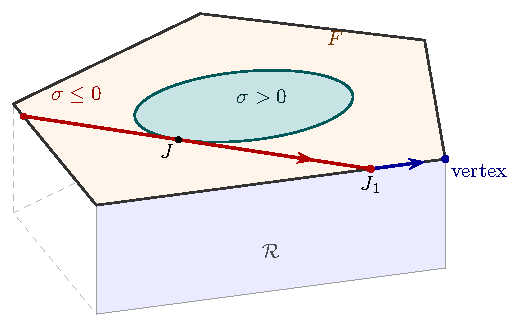
\includegraphics[width=0.78\textwidth]{figures/descent}
\caption{One step of the proof of Proposition~\ref{prop:descent} in a two-dimensional face $F$ of $\Rk$, in case (b), $\sigma(J)=0$. The set $F\cap\{\sigma>0\}$ (shaded) is convex because $\sigma$ is concave. On the line through $J$ in the direction $X$, chosen with $X[u]=0$, we have $\sigma\le0$, and $\log\det Q$ is concave on it, so one of the two ends of the chord, here $J_1$, has $\det Q(J_1)\le\det Q(J)$. The point $J_1$ lies on an edge of $F$. From there the same step moves along the edge to a vertex or to a point with $\sigma=0$.}
\label{fig:descent}
\end{figure}

\section{The vertices and edges of \texorpdfstring{$\Rk$}{R}}\label{sec:computation}

\begin{definition}\label{def:Xua}
For $u\in\Z^5$ and $a\in\Z$ let $p=(u,-a)$, $q=(u,-a-1)\in\Z^6$ and $X_{u,a}=pq^\T+qp^\T$. Thus $Q(X_{u,a})=2uu^\T$ and
\[
X_{u,a}[(n,l)]=2\,(u\cdot n-al)\,(u\cdot n-(a+1)l).
\]
\end{definition}

\begin{lemma}\label{lem:Xua}
$X_{u,a}[k]\ge0$ for all $k\in\M$. Hence $J+tX_{u,a}\in\Rk$ for all $J\in\Rk$ and $t\ge0$, and
\[
\det Q(J+tX_{u,a})=\det Q(J)+2t\,\adj(Q(J))[u].
\]
\end{lemma}

\begin{proof}
For $k=(n,l)$ the two factors $u\cdot n-al$ and $u\cdot n-(a+1)l$ are integers that differ by $l\in\{-1,0,1\}$; two such integers have a nonnegative product. The determinant formula is the matrix determinant lemma for the rank-one update $Q+2t\,uu^\T$.
\end{proof}

\begin{table}[t]
\centering
\small
\renewcommand{\arraystretch}{1.05}
\setlength{\tabcolsep}{4.5pt}
\begin{tabular}{@{}r r r r r r r c r r r r r r r@{}}
\toprule
$i$ & $|\Min|$ & $\det Q$ & $\det J$ & rays & orb. & U & \hspace{6pt} & $i$ & $|\Min|$ & $\det Q$ & $\det J$ & rays & orb. & U\\
\cmidrule(r){1-7}\cmidrule(l){9-15}
0 & 32 & 512 & 0 & 1166 & 22 & 2 & & 17 & 21 & 294 & 343 & 21 & 4 & 0 \\
1 & 37 & 1024 & $-1024$ & 373 & 7 & 1 & & 18 & 21 & 288 & 351 & 21 & 8 & 1 \\
2 & 30 & 768 & $-256$ & 148 & 9 & 1 & & 19 & 22 & 234 & 324 & 46 & 15 & 1 \\
3 & 31 & 320 & 192 & 2621 & 38 & 2 & & 20 & 21 & 252 & 351 & 21 & 10 & 0 \\
4 & 24 & 512 & 256 & 56 & 6 & 1 & & 21 & 21 & 384 & 448 & 21 & 3 & 0 \\
5 & 36 & 128 & 192 & 38124 & 72 & 2 & & 22 & 30 & 128 & 256 & 6336 & 20 & 1 \\
6 & 25 & 324 & 243 & 261 & 11 & 1 & & 23 & 27 & 162 & 243 & 621 & 11 & 1 \\
7 & 29 & 256 & 256 & 2273 & 23 & 2 & & 24 & 22 & 216 & 324 & 46 & 11 & 0 \\
8 & 35 & 192 & 192 & 21196 & 56 & 2 & & 25 & 22 & 180 & 324 & 46 & 11 & 0 \\
9 & 24 & 432 & 216 & 56 & 8 & 1 & & 26 & 22 & 162 & 324 & 46 & 6 & 0 \\
10 & 21 & 378 & 324 & 21 & 11 & 1 & & 27 & 21 & 180 & 351 & 21 & 8 & 0 \\
11 & 30 & 192 & 256 & 6336 & 40 & 1 & & 28 & 21 & 196 & 343 & 21 & 4 & 0 \\
12 & 27 & 384 & 256 & 515 & 14 & 1 & & 29 & 21 & 216 & 351 & 21 & 6 & 0 \\
13 & 25 & 576 & 192 & 64 & 6 & 1 & & 30 & 21 & 234 & 351 & 21 & 6 & 0 \\
14 & 22 & 288 & 324 & 46 & 11 & 0 & & 31 & 21 & 162 & 351 & 21 & 3 & 0 \\
15 & 22 & 324 & 324 & 46 & 5 & 1 & & 32 & 21 & 320 & 448 & 21 & 3 & 1 \\
16 & 21 & 306 & 351 & 21 & 10 & 0 & & 33 & 21 & 192 & 448 & 21 & 2 & 0 \\
\bottomrule
\end{tabular}
\caption{The $34$ vertices $J_i$ of $\Rk$ up to equivalence; their entries are in Table~\ref{tab:J}. $|\Min|$ counts pairs $\pm k$; ``rays'' is the number of extreme rays of $C_{J_i}$, ``orb.'' the number of their orbits under the group $G_i\subseteq\Gamma_{J_i}$ generated by the automorphisms of $J_i$ listed in the certificate, and U the number of these orbits that are unbounded edges. In all, $80{,}695$ rays in $480$ orbits, $25$ of them unbounded. The pairs $(\det Q,\det J)$ are distinct, so no two $J_i$ are equivalent.}
\label{tab:vertices}
\end{table}

\begin{proposition}\label{prop:computation}
The matrices $J_0,\dots,J_{33}$ of Table~\ref{tab:J} are vertices of $\Rk$ with the invariants of Table~\ref{tab:vertices}. For each $i$ let $G_i$ be as in Table~\ref{tab:vertices}. Then:
\begin{enumerate}
\item for every extreme ray $Y$ of $C_{J_i}$ with $t^*(J_i,Y)<\infty$, the vertex $J_i+t^*Y$ is equivalent to some $J_j$; Table~\ref{tab:edges} lists $j$ for one ray of each $G_i$-orbit;
\item for every extreme ray $Y$ of $C_{J_i}$ and every $t\ge0$ with $t\le t^*(J_i,Y)$, either $\det(J_i+tY)>0$ or $\det Q(J_i+tY)\ge512$; and if $\det(J_i+tY)=0$ and $\det Q(J_i+tY)=512$, then $J_i+tY$ is equivalent to one of the matrices $E_0,\dots,E_4$ of Proposition~\ref{prop:candidates};
\item every extreme ray $Y$ of $C_{J_i}$ with $t^*(J_i,Y)=\infty$ equals $X_{u,a}$ for some $u\in\Z^5$ and $a\in\{-2,-1,0\}$, and is $G_i$-equivalent to one of the $25$ rays of Table~\ref{tab:unbounded}.
\end{enumerate}
\end{proposition}

\begin{proof}
This is a finite computation in exact integer and rational arithmetic, described in Appendix~\ref{app:verification}. The certificate lists, for each $i$, the minimal vectors of $J_i$, generators of $G_i$, all extreme rays of $C_{J_i}$, and one ray $Y$ of each $G_i$-orbit; for a bounded edge it gives $t^*$, $j$ and a matrix $T\in\Gamma$ with $T^\T J_jT=J_i+t^*Y$, and for an unbounded edge the data $(u,a)$. For a ray $gYg^\T$ with $g\in G_i$, the edge at $J_i$ in its direction is the image of the edge in direction $Y$ under $J\mapsto g^\T Jg$ (Section~\ref{ssec:symmetries}), so the statements for the listed rays imply them for all rays. Statement (2) is decided on each listed edge from the polynomials $\det(J_i+tY)$, of degree at most $6$, and $\det Q(J_i+tY)$, of degree at most $5$, by Sturm sequences.
\end{proof}

By Corollary~\ref{cor:closure} and Proposition~\ref{prop:computation}(1), every vertex of $\Rk$ is equivalent to exactly one $J_i$, and every edge of $\Rk$ is equivalent to an edge at some $J_i$ in the direction of one of the $480$ listed rays.

\begin{table}[t]
\centering
\small
\renewcommand{\arraystretch}{1.18}
\setlength{\tabcolsep}{4pt}
\begin{tabular}{@{}r l r l l l l@{}}
\toprule
$i$ & $(u,a)$ & $N$ & $\det Q(J_i+tX_{u,a})$ & $\det(J_i+tX_{u,a})$ & $t_0$ & $\det Q$ at $t_0$\\
\midrule
0 & $(e_2,-1)$ & 4 & $128(3t+4)$ & $-64t(3t+4)$ & --- & ---\\
0 & $(e_4,0)$ & 2 & $256(t+2)$ & $-128t(t+2)$ & --- & ---\\
1 & $(e_1,-1)$ & 5 & $512(t+2)$ & $-256(t+2)^2$ & --- & ---\\
2 & $(e_2,-1)$ & 3 & $384(t+2)$ & $-64(t+2)(3t+2)$ & --- & ---\\
3 & $((1,-1,-1,0,0),-1)$ & 5 & $64(4t+5)$ & $-64(2t^2-3)$ & $\sqrt6/2$ & $320+128\sqrt6$\\
3 & $(e_1,-1)$ & 1 & $160(t+2)$ & $-16(t+2)(5t-6)$ & $6/5$ & $512$\\
4 & $(e_4,0)$ & 2 & $256(t+2)$ & $-128(t-1)(t+2)$ & $1$ & $768$\\
5 & $(e_1,-1)$ & 16 & $32(5t+4)$ & $-16(5t^2-12t-12)$ & $(6+4\sqrt6)/5$ & $320+128\sqrt6$\\
5 & $(e_5,0)$ & 5 & $128(t+1)$ & $-64(t-3)(t+1)$ & $3$ & $512$\\
6 & $(e_5,0)$ & 4 & $108(2t+3)$ & $-27(2t-3)(2t+3)$ & $3/2$ & $648$\\
7 & $((1,1,0,-1,0),-2)$ & 8 & $256(t+1)$ & $-128(t-2)(t+1)$ & $2$ & $768$\\
7 & $(e_5,0)$ & 1 & $128(t+2)$ & $-64(t-2)(t+2)$ & $2$ & $512$\\
8 & $((0,1,1,0,1),0)$ & 10 & $96(3t+2)$ & $-48(t-2)(3t+2)$ & $2$ & $768$\\
8 & $(e_1,-1)$ & 6 & $32(5t+6)$ & $-16(t-2)(5t+6)$ & $2$ & $512$\\
9 & $(e_5,0)$ & 1 & $216(t+2)$ & $-108(t-1)(t+2)$ & $1$ & $648$\\
10 & $(e_5,0)$ & 1 & $54(4t+7)$ & $-108(t^2-3)$ & $\sqrt3$ & $378+216\sqrt3$\\
11 & $(e_4,0)$ & 6 & $32(5t+6)$ & $-16(5t^2-8t-16)$ & $(4+4\sqrt6)/5$ & $320+128\sqrt6$\\
12 & $(e_2,-1)$ & 4 & $96(3t+4)$ & $-16(3t-4)(3t+4)$ & $4/3$ & $768$\\
13 & $(e_2,-1)$ & 1 & $288(t+2)$ & $-48(t+2)(3t-2)$ & $2/3$ & $768$\\
15 & $(e_1,-1)$ & 1 & $162(t+2)$ & $-81(t-2)(t+2)$ & $2$ & $648$\\
18 & $(e_1,-1)$ & 1 & $18(9t+16)$ & $-27(3t^2-2t-13)$ & $(1+2\sqrt{10})/3$ & $342+108\sqrt{10}$\\
19 & $(e_1,-1)$ & 1 & $18(9t+13)$ & $-27(3t^2-4t-12)$ & $(2+2\sqrt{10})/3$ & $342+108\sqrt{10}$\\
22 & $(e_1,-1)$ & 16 & $32(5t+4)$ & $-16(t-4)(5t+4)$ & $4$ & $768$\\
23 & $((0,1,0,-1,-1),-2)$ & 10 & $162(t+1)$ & $-81(t-3)(t+1)$ & $3$ & $648$\\
32 & $(e_5,0)$ & 1 & $160(t+2)$ & $-16(t+2)(5t-14)$ & $14/5$ & $768$\\
\bottomrule
\end{tabular}
\caption{The unbounded edges $J_i+tX_{u,a}$, $t\ge0$, one per $G_i$-orbit; $N$ is the size of the orbit, and the $N$ add up to $115$. The last two columns give the positive root $t_0$ of $\det(J_i+tX_{u,a})$ and the value of $\det Q$ there. Each row is a direct computation from Table~\ref{tab:J} (the $\det Q$ column by Lemma~\ref{lem:Xua}); $320+128\sqrt6\approx633.5$, $342+108\sqrt{10}\approx683.5$, $378+216\sqrt3\approx752.1$.}
\label{tab:unbounded}
\end{table}

\begin{remark}\label{rem:bounded}
The concavity of $\sigma$ (Lemma~\ref{lem:sigma}(2)) locates the points of $\cand$ on bounded edges. By Table~\ref{tab:vertices}, $\sigma(J_i)$ is negative for $i=1,2$, zero for $i=0$ and positive otherwise. On a bounded edge whose end points have $\sigma\ge0$, not both zero, $\sigma$ is positive inside. So a point of $\cand$ in the interior of a bounded edge lies on an edge at $J_1$ or $J_2$, or on an edge joining two vertices of class $0$. There are two classes of the latter. On one, $\det J=16t(t-4)(t-2)(t+2)$ with $t^*=2$, which is positive inside. On the other, $\det J\equiv0$ and $\det Q=512(1+\tau-\tau^2)$ with $\tau=t/t^*$; this is the edge of~\cite[\S4.3]{AK2020} contained in the set of packings, with $\det Q>512$ inside. On ten classes of edges at $J_1$ or $J_2$, $\det J$ has one root inside, where $\det Q$ equals $648$, $673.59\ldots$, $697.00\ldots$, $711.11\ldots$, $714.19\ldots$, $715.45\ldots$, $734.56\ldots$, $737.28$, $738.50\ldots$ and $823.04\ldots$ respectively; on the other edges at $J_1$ and $J_2$, $\det J<0$ inside. Proposition~\ref{prop:computation}(2) records these facts; they are not used separately.
\end{remark}

\begin{proposition}\label{prop:candidates}
Let
\[
E_0=J_0,\quad E_1=J_3+\tfrac65X_{e_1,-1},\quad E_2=J_5+3X_{e_5,0},\quad E_3=J_7+2X_{e_5,0},\quad E_4=J_8+2X_{e_1,-1}.
\]
Every $J\in\cand$ satisfies $\det Q(J)\ge512$, with equality if and only if $J$ is equivalent to one of $E_0,\dots,E_4$.
\end{proposition}

\begin{proof}
Let $J\in\cand$. If $d(J)=0$, then $J$ is equivalent to some $J_i$ with $\sigma(J_i)\le0$, that is, $\det J_i\le0$. By Table~\ref{tab:vertices}, $i\in\{0,1,2\}$ and $\det Q(J)\in\{512,1024,768\}$, with $512$ only for $J_0=E_0$.

If $d(J)=1$ and $\sigma(J)=0$, Lemma~\ref{lem:edges}(3) places $J$ in the relative interior of an edge, and after applying an element of $\Gamma$ we may assume $J=J_i+tY$ with $Y$ an extreme ray of $C_{J_i}$ and $0<t<t^*(J_i,Y)$. Then $\det J=\det Q(J)\,\sigma(J)=0$, and Proposition~\ref{prop:computation}(2) gives $\det Q(J)\ge512$, with equality only if $J$ is equivalent to some $E_m$.

Conversely, $E_0=J_0$ is a vertex with $\det J_0=0$ and $\det Q(J_0)=512$. For $m\ge1$, $E_m$ is the point at $t_0$ on one of the four rows of Table~\ref{tab:unbounded} with $\det Q(t_0)=512$; it lies in the relative interior of an unbounded edge, so $d(E_m)=1$ by Lemma~\ref{lem:edges}(2), and $\sigma(E_m)=\det E_m/\det Q(E_m)=0$.
\end{proof}

\begin{corollary}\label{cor:bound}
$\det Q(J)\ge512$ for every $J\in S$.
\end{corollary}

\begin{proof}
Propositions~\ref{prop:descent} and~\ref{prop:candidates}.
\end{proof}

\section{The equality case}\label{sec:equality}

\begin{lemma}\label{lem:deephole}
Let $\Lambda\subset\R^n$ be a lattice, $\rho=\max_{z\in\R^n}\dist(z,\Lambda)$ its covering radius, and $c\in\R^n$ with $\dist(c,\Lambda)=\rho$. Then the set $N(c)=\{v\in\Lambda:|v-c|=\rho\}$ is not contained in any affine hyperplane.
\end{lemma}

\begin{proof}
The maximum exists because $z\mapsto\dist(z,\Lambda)$ is continuous and $\Lambda$-periodic. $N(c)$ is finite and nonempty, and since $\Lambda$ is discrete there is $\delta>0$ with $|v-c|\ge\rho+\delta$ for $v\in\Lambda\setminus N(c)$. Suppose $\langle v,z\rangle=\alpha$ for all $v\in N(c)$, with $|z|=1$. Put $\beta=\alpha-\langle c,z\rangle$, so that $\langle v-c,z\rangle=\beta$ on $N(c)$, and let $w=-z$ if $\beta>0$ and $w=z$ otherwise. For $0<\varepsilon<\delta$ and $v\in N(c)$,
\[
|v-c-\varepsilon w|^2=\rho^2-2\varepsilon\langle v-c,w\rangle+\varepsilon^2=\rho^2+2\varepsilon|\beta|+\varepsilon^2>\rho^2,
\]
and for $v\in\Lambda\setminus N(c)$, $|v-c-\varepsilon w|\ge\rho+\delta-\varepsilon>\rho$. So $\dist(c+\varepsilon w,\Lambda)>\rho$, contradicting the definition of $\rho$.
\end{proof}

\begin{figure}[t]
\centering
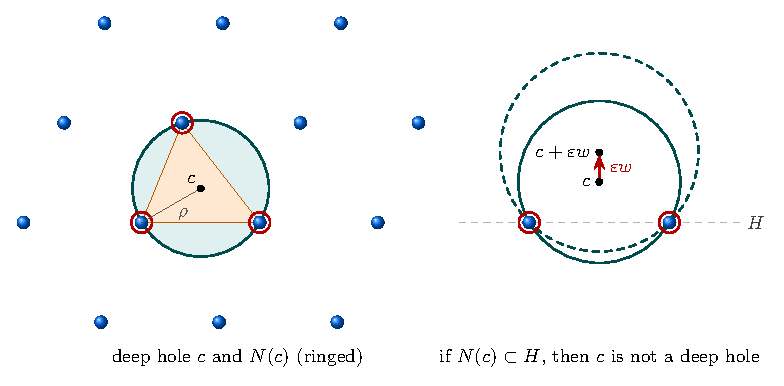
\includegraphics[width=0.9\textwidth]{figures/deephole}
\caption{Lemma~\ref{lem:deephole} in the plane. Left: a deep hole $c$ of a lattice; the open disc of radius $\rho$ about $c$ contains no lattice point, and the points $N(c)$ on its boundary span the plane affinely. Right: if $N(c)$ lay on a line $H$, moving $c$ away from $H$ by a small $\varepsilon w$ would increase the distance to every point of $N(c)$, and to the whole lattice, beyond $\rho$.}
\label{fig:deephole}
\end{figure}

A point $c$ with $\dist(c,\Lambda)=\rho$ is a \emph{deep hole} of $\Lambda$.

\begin{lemma}\label{lem:dictionary}
Let $J\in\Sym_6^+$, let $A$ be a real $5\times5$ matrix with $A^\T A=Q(J)$, and put $\Lambda=A\Z^5$ and $c=-Aq(J)$. Then $J[(n,0)]=|An|^2$ and $J[(n,1)]=|An-c|^2+\sigma(J)$ for $n\in\Z^5$. In particular $J\in\Rk$ if and only if $|v|\ge2$ for $v\in\Lambda\setminus0$ and $\dist(c,\Lambda)^2\ge4-\sigma(J)$; and for $J\in\Rk$ we have $(n,1)\in\Min(J)$ if and only if $|An-c|^2=4-\sigma(J)$.
\end{lemma}

\begin{proof}
By Lemma~\ref{lem:sigma}(1), $J[(n,l)]=|A(n+lq(J))|^2+l^2\sigma(J)=|An-lc|^2+l^2\sigma(J)$. The vectors $(n,-1)$ give the same values as $(-n,1)$.
\end{proof}

\begin{proposition}\label{prop:equality}
Let $J\in S$ with $\det Q(J)=512$. Then $\sigma(J)=0$ and $d(J)\le1$. Hence $J\in\cand$, and $J$ is equivalent to one of $E_0,\dots,E_4$.
\end{proposition}

\begin{proof}
We first record two consequences of Corollary~\ref{cor:bound} for any $J'\in S$ with $\det Q(J')=512$ and any $X\in L_{J'}$ that satisfies $\sigma(J')<0$ or $X[u']=0$, where $u'=(-q(J'),1)$:
\begin{enumerate}
\item[(a)] $Q(X)=0$;
\item[(b)] writing $X=\left(\begin{smallmatrix}0&x\\x^\T&y\end{smallmatrix}\right)$, we have $2x\cdot n+y=0$ for every $(n,1)\in\Min(J')$.
\end{enumerate}
For (a): $J'+\tau X\in\Rk$ for small $|\tau|$ by Lemma~\ref{lem:local}(2), since $\pm X\in C_{J'}$. If $\sigma(J')<0$, then $\sigma(J'+\tau X)<0$ for small $|\tau|$ by continuity. If $X[u']=0$, then $\sigma(J'+\tau X)\le(J'+\tau X)[u']=\sigma(J')\le0$ by Lemma~\ref{lem:sigma}(2). In both cases $J'+\tau X\in S$ on an interval around $0$, where $\varphi(\tau)=\log\det Q(J'+\tau X)$ is concave, at least $\log512$ by Corollary~\ref{cor:bound}, and equal to $\log512$ at $\tau=0$. A concave function with an interior minimum on an interval is constant there, so $Q(X)=0$ by Lemma~\ref{lem:logdet}. For (b): with $Q(X)=0$ we have $X[(n,1)]=2x\cdot n+y$, which vanishes on $\Min(J')$ because $X\in L_{J'}$.

Now let $J$ be as in the proposition, and let $A$, $\Lambda$, $c$ be as in Lemma~\ref{lem:dictionary}. Let $\rho$ be the covering radius of $\Lambda$. Since $J\in\Rk$ and $\sigma(J)\le0$, Lemma~\ref{lem:dictionary} gives $\rho^2\ge\dist(c,\Lambda)^2\ge4-\sigma(J)\ge4$.

Suppose $\rho>2$. Choose a deep hole $c'$ of $\Lambda$, put $q'=-A^{-1}c'$ and $\sigma'=4-\rho^2<0$, and let
\[
J'=\begin{pmatrix}Q&Qq'\\ q'^\T Q&\sigma'+Q[q']\end{pmatrix},\qquad Q=Q(J).
\]
Then $Q(J')=Q$, $q(J')=q'$ and $\sigma(J')=\sigma'$. By Lemma~\ref{lem:dictionary}, $J'\in\Rk$, because $\Lambda$ has minimal distance at least $2$ and $\dist(c',\Lambda)^2=\rho^2=4-\sigma'$; moreover $(n,1)\in\Min(J')$ whenever $An\in N(c')$. So $J'\in S$ and $\det Q(J')=512$. Let $X\in L_{J'}$. Since $\sigma(J')<0$, (a) and (b) apply: $Q(X)=0$, and the affine function $v\mapsto2x\cdot A^{-1}v+y$ vanishes on $N(c')$. By Lemma~\ref{lem:deephole}, $N(c')$ is not contained in an affine hyperplane, so $x=0$ and $y=0$, that is, $X=0$. Hence $d(J')=0$: $J'$ is a vertex with $\det J'=512\,\sigma'<0$. By Proposition~\ref{prop:computation} it is equivalent to $J_1$ or $J_2$, the only $J_i$ with $\det J_i<0$; but $\det Q(J_1)=1024$ and $\det Q(J_2)=768$. This contradiction shows $\rho=2$.

Then $4\ge\dist(c,\Lambda)^2\ge4-\sigma(J)$ gives $\sigma(J)=0$ and $\dist(c,\Lambda)=2=\rho$, so $c$ is a deep hole of $\Lambda$, and $(n,1)\in\Min(J)$ if and only if $An\in N(c)$. Let $u=(-q(J),1)$ and let $X\in L_J$ with $X[u]=0$. By (a) and (b), $Q(X)=0$ and $v\mapsto2x\cdot A^{-1}v+y$ vanishes on $N(c)$, so $X=0$ by Lemma~\ref{lem:deephole}. Thus the linear map $L_J\to\R$, $X\mapsto X[u]$, is injective, and $d(J)\le1$. So $J\in\cand$, and Proposition~\ref{prop:candidates} completes the proof.
\end{proof}

\section{The five extremal configurations}\label{sec:five}

\begin{table}[t]
\centering
\small
\renewcommand{\arraystretch}{1.25}
\begin{tabular}{@{}c l l@{}}
\toprule
$m$ & $a_1,\ a_2,\ a_3,\ a_4,\ a_5$ & $b$\\
\midrule
0 & $(0\,1\,\bar{1}\,0\,0)$\ $(1\,0\,1\,0\,0)$\ $(1\,\bar{1}\,0\,0\,0)$\ $(0\,0\,0\,1\,\bar{1})$\ $(0\,0\,0\,1\,1)$ & $(0\,1\,0\,\bar{1}\,0)$ \\
1 & $\tfrac1{5}(1\,\bar{9}\,\bar{4}\,\bar{4}\,\bar{4})$\ $(\bar{1}\,0\,0\,0\,1)$\ $(\bar{1}\,1\,0\,0\,0)$\ $(0\,\bar{1}\,0\,1\,0)$\ $(0\,\bar{1}\,1\,0\,0)$ & $\tfrac1{5}(1\,\bar{4}\,\bar{4}\,\bar{4}\,1)$ \\
2 & $(1\,0\,1\,0\,0)$\ $(0\,1\,0\,1\,0)$\ $(0\,0\,\bar{1}\,1\,0)$\ $(0\,0\,\bar{1}\,\bar{1}\,0)$\ $-\tfrac1{2}(1\,1\,1\,1\,4)$ & $(1\,1\,2\,1\,1)$ \\
3 & $(0\,1\,0\,\bar{1}\,0)$\ $(1\,0\,\bar{1}\,0\,0)$\ $(1\,\bar{1}\,0\,0\,0)$\ $(0\,0\,1\,1\,0)$\ $(0\,0\,0\,0\,2)$ & $(0\,1\,\bar{1}\,\bar{1}\,\bar{1})$ \\
4 & $(\bar{1}\,\bar{1}\,\bar{1}\,0\,\bar{1})$\ $(0\,1\,0\,0\,\bar{1})$\ $(0\,1\,0\,\bar{1}\,0)$\ $(1\,\bar{1}\,0\,0\,0)$\ $(0\,0\,1\,\bar{1}\,0)$ & $(\bar{1}\,0\,\bar{1}\,1\,\bar{1})$ \\
\bottomrule
\end{tabular}
\caption{Bases of $\Lambda_m$ and vectors $b\equiv b_m\pmod{\Lambda_m}$; the Gram matrix of $\sqrt2\,(a_1,\dots,a_5,b)$ is $E_m$. Coordinates are written without commas, and $\bar k=-k$.}
\label{tab:vectors}
\end{table}

\begin{lemma}\label{lem:vectors}
For each $m$, the vectors $a_1,\dots,a_5$ of Table~\ref{tab:vectors} form a basis of $\Lambda_m$, the vector $b$ satisfies $b-b_m\in\Lambda_m$, and the Gram matrix of $\sqrt2\,a_1,\dots,\sqrt2\,a_5,\sqrt2\,b$ is $E_m$. Each $\Lambda_m$ has covolume $4$, minimal norm $2$ and $|\Min\Lambda_m|$ as in Table~\ref{tab:five}.
\end{lemma}

\begin{proof}
$\Lambda_0$, $\Lambda_3$ and $\Lambda_4$ have index $4$ in $\Z^5$. $\Lambda_1$ is the orthogonal sum of $A_4$, of determinant $5$, and $\Z\frac45\one$, of norm $\frac{16}5$; $\Lambda_2$ consists of the layers $x_5=2j$, each a translate of $D_4$, of covolume $2$, at spacing $2$. So all five have covolume $4$. The vectors $a_i$ lie in $\Lambda_m$ and $|\det(a_1,\dots,a_5)|=4$, so they form a basis; $b-b_m\in\Lambda_m$ and the Gram matrices are direct computations. The norm-$2$ vectors are: the $4\cdot3+4\cdot1=16$ vectors $\pm e_i\pm e_j$ of $D_3\oplus D_2$; the $20$ roots of $A_4$, since $\Lambda_1$ has no other vector of norm less than $\frac{16}5$; the $24$ roots of $D_4\times0$, since a vector of $\Lambda_2$ with $x_5=2j\ne0$ has norm at least $1+4=5$; the $24$ roots of $D_4\times0$ in $\Lambda_3$; and the $20$ vectors $e_i-e_j$ in $\Lambda_4$.
\end{proof}

\begin{lemma}\label{lem:noncongruent}
\begin{enumerate}
\item $P_0=P_3=P_4=D_5$.
\item For $m=1,2$, $2b_m\notin\Lambda_m$; the set $P_m$ is not a lattice, and its group of translations $\{y:P_m+y=P_m\}$ is $\Lambda_m$.
\item The five pairs $(\Lambda_m,b_m)$ are pairwise not congruent, and $P_1$, $P_2$, $D_5$ are pairwise not congruent.
\end{enumerate}
\end{lemma}

\begin{proof}
(1) $\Lambda_m\subset D_5$ for $m=0,3,4$, with index $2$ since $\covol(D_5)=2$, and $b_m\in D_5\setminus\Lambda_m$. So $P_m$ is the union of the two cosets of $\Lambda_m$ in $D_5$.
(2) $2b_1=2e_1+2e_5$ has coordinate sum $4$, so its component along $\one$ is $\frac45\one$, and $2b_1-\frac45\one=\frac25(3,-2,-2,-2,3)\notin\Z^5$; so $2b_1\notin\Lambda_1$. $2b_2=2e_1+2e_5$ has $x_5=2$, while the vectors of $\Lambda_2$ with $x_5=2$ lie in $(D_4+h)\times\{2\}$, which does not contain $2e_1$. Let $y$ be a translation of $P=\Lambda\cup(\Lambda+b)$, where $b\notin\Lambda$ and $2b\notin\Lambda$. Then $y=0+y\in P$. If $y\in\Lambda+b$, then $y+b\in\Lambda+2b$, which meets neither $\Lambda$ nor $\Lambda+b$. So $y\in\Lambda$, and conversely every $y\in\Lambda$ is a translation. As $P\ne\Lambda$, $P$ is not a lattice.
(3) A congruence of pairs maps $\Lambda$ onto $\Lambda'$, so it preserves $|\Min\Lambda|$, and it preserves whether $2b\in\Lambda$. The pairs $(|\Min\Lambda_m|,[2b_m\in\Lambda_m])$ are $(16,1)$, $(20,0)$, $(24,0)$, $(24,1)$, $(20,1)$, all distinct. A congruence of point sets carries the group of translations of one onto that of the other. $D_5$ is a lattice and $P_1,P_2$ are not, and a congruence $P_1\to P_2$ would map $\Lambda_1$ onto $\Lambda_2$, which have $20$ and $24$ vectors of minimal norm.
\end{proof}

\begin{remark}\label{rem:identify}
(1) Every splitting of $D_5$ into the two cosets of a sublattice of index two satisfies the packing condition, so the theorem lists each such splitting up to congruence. $D_5$ has $31$ sublattices of index two, the kernels of the $31$ nonzero homomorphisms $D_5\to\Z/2$: $x\mapsto x_i$, $x\mapsto x_i+x_j$ and $x\mapsto\frac12\sum_i\varepsilon_ix_i$ modulo $2$, with $\varepsilon\in\{\pm1\}^5$ up to sign; there are $5$, $10$ and $16$ of them. Signed permutations of the coordinates map them to $\Lambda_3$, $\Lambda_0$ and $\Lambda_4$ respectively.

(2) Translations by $\Lambda$ and the point reflection $x\mapsto b-x$ preserve $P=\Lambda\cup(\Lambda+b)$, and together they act transitively on $P$, so every packing of the theorem is uniform. In $P_1$ and $P_2$ every point has $40$ neighbours at distance $\sqrt2$. The isometry $x\mapsto-(x_4,x_2,x_3,x_1,x_5)$ maps $\Lambda_1$ onto itself and $b_1$ onto $-e_4-e_5$, so it maps $P_1$ onto the packing given by the lattice basis $e_1-e_2,\dots,e_4-e_5,\frac45\one$ and the translation vectors $0$, $(0,0,0,-1,-1)$ in~\cite[Table~4.2]{CR2026}: the uniform packing with kissing configuration $Q_5$, which is $J_{5,5}$ of~\cite{AK2020}~\cite[\S1]{CR2026}.

(3) $P_2=\bigcup_{i\in\Z}(D_4+c_i)\times\{i\}$ with $c_i=0$, $e_1$, $h$, $e_1+h$ for $i\equiv0,1,2,3\pmod4$. The neighbours of $0$ are the $24$ roots of $D_4$ in the layer $i=0$, the $8$ points $(\pm e_k,1)$, $1\le k\le4$, and the $8$ points $(\frac12(\pm1,\pm1,\pm1,\pm1),-1)$ with an odd number of minus signs. This is Leech's configuration $L_5$~\cite{Leech1967}, as described in~\cite[\S2]{CR2026}, reflected in the hyperplane $x_5=0$. By Lemma~\ref{lem:noncongruent}(2), $P_2$ is $2$-periodic in the sense of~\cite{CR2026}, so by~\cite[Theorem~4.3]{CR2026} and~\cite[\S5]{CS1995}, $\sqrt2\,P_2$ is the $2$-periodic one of Leech's three uniform packings.
\end{remark}

\section{Proofs of Theorem~\ref{thm:main} and Corollary~\ref{cor:cells}}\label{sec:proofs}

\begin{proof}[Proof of Theorem~\ref{thm:main}]
Let $\Lambda$ and $b$ be as in the theorem, $a$ a basis of $\Lambda$ and $J=J(a,b)$. By Lemmas~\ref{lem:packing} and~\ref{lem:rank5}, $J\in\Rk$ and $\sigma(J)=0$, so $J\in S$, and $\det Q(J)=\covol(\Lambda)^2$. Corollary~\ref{cor:bound} gives $\covol(\Lambda)\ge\sqrt{512}=16\sqrt2$.

If $\covol(\Lambda)=16\sqrt2$, then $\det Q(J)=512$, and Proposition~\ref{prop:equality} shows that $J$ is equivalent to some $E_m$. By Lemma~\ref{lem:vectors}, $E_m=J(\sqrt2\,a^{(m)},\sqrt2\,b^{(m)})$, where $a^{(m)},b^{(m)}$ are the vectors of Table~\ref{tab:vectors}, $a^{(m)}$ is a basis of $\Lambda_m$ and $\Lambda_m+b^{(m)}=\Lambda_m+b_m$. By Lemma~\ref{lem:congruent}, $(\Lambda,b)$ is congruent to $(\sqrt2\,\Lambda_m,\sqrt2\,b_m)$.

Conversely, $E_m\in\cand\subset\Rk$ and $\sigma(E_m)=0$ (Proposition~\ref{prop:candidates}), so by Lemmas~\ref{lem:rank5} and~\ref{lem:vectors} the pair $(\sqrt2\,\Lambda_m,\sqrt2\,b_m)$ satisfies the hypotheses: $b_m\notin\Lambda_m$, and $\covol(\sqrt2\,\Lambda_m)^2=\det Q(E_m)=512$. The five pairs are pairwise not congruent by Lemma~\ref{lem:noncongruent}(3).

Finally, $P$ has two points per fundamental domain of $\Lambda$, so the density of the packing of unit balls centred at $P$ is $2\cdot\frac{8\pi^2}{15}/\covol(\Lambda)\le\pi^2/(15\sqrt2)$. Equality holds exactly when $(\Lambda,b)$ is congruent to some $(\sqrt2\,\Lambda_m,\sqrt2\,b_m)$, that is, when $P$ is congruent to some $\sqrt2\,P_m$; by Lemma~\ref{lem:noncongruent}, these sets are $\sqrt2\,D_5$, $\sqrt2\,P_1$ and $\sqrt2\,P_2$.
\end{proof}

\begin{proof}[Proof of Corollary~\ref{cor:cells}]
If $P=L$ is a lattice with basis $l_1,\dots,l_5$, let $\Lambda$ be the sublattice of index two spanned by $2l_1,l_2,\dots,l_5$ and $b=l_1$; then $P=\Lambda\cup(\Lambda+b)$. So in both cases $P=\Lambda\cup(\Lambda+b)$ with $b\notin\Lambda$. The map $x\mapsto b-x$ is an isometry of $P$ exchanging $\Lambda$ and $\Lambda+b$; it maps the Voronoi cell $V_0$ of $0$ onto the cell $V_b$ of $b$. Translations by $\Lambda$ permute the cells, and $V_0\cup V_b$ is a fundamental domain of $\Lambda$ up to a null set. Hence every cell has volume $\frac12\covol(\Lambda)\ge8\sqrt2$ by Theorem~\ref{thm:main}, with equality exactly for the sets listed there. The Voronoi cell of $\sqrt2\,D_5$ has volume $\covol(\sqrt2\,D_5)=2\cdot2^{5/2}=8\sqrt2$.
\end{proof}

\appendix

\section{Tables}\label{app:tables}

\begin{table}[h]
\centering
\scriptsize
\renewcommand{\arraystretch}{1.08}
\setlength{\tabcolsep}{2.1pt}
\begin{tabular}{@{}>{$}l<{$}*{21}{>{$}r<{$}}@{}}
\toprule
 & 11 & 12 & 13 & 14 & 15 & 16 & 22 & 23 & 24 & 25 & 26 & 33 & 34 & 35 & 36 & 44 & 45 & 46 & 55 & 56 & 66\\
\midrule
J_{0} & 4 & -2 & -2 & 0 & 0 & 2 & 4 & 2 & 0 & 0 & 0 & 4 & 0 & 0 & -2 & 4 & 0 & -2 & 4 & -2 & 4 \\
J_{1} & 4 & 0 & 0 & 0 & 0 & 2 & 4 & 0 & 0 & 0 & 2 & 4 & 0 & 0 & -2 & 4 & 0 & -2 & 4 & -2 & 4 \\
J_{2} & 4 & 0 & -2 & 0 & 0 & 4 & 4 & 0 & 0 & 0 & 2 & 4 & 0 & 0 & -4 & 4 & 0 & -2 & 4 & -2 & 8 \\
J_{3} & 8 & -2 & -4 & 2 & 2 & 4 & 4 & 2 & 0 & 0 & 0 & 4 & -2 & -2 & -2 & 4 & 2 & 0 & 4 & 0 & 4 \\
J_{4} & 4 & 0 & -2 & 0 & 0 & 4 & 4 & 2 & 0 & 0 & 2 & 4 & 0 & 0 & -2 & 4 & 0 & -2 & 4 & -2 & 8 \\
J_{5} & 4 & 0 & -2 & -2 & -2 & 6 & 4 & 2 & -2 & -2 & 4 & 4 & 0 & 0 & -2 & 4 & 2 & -6 & 4 & -6 & 16 \\
J_{6} & 4 & -1 & -2 & 1 & 1 & 1 & 4 & 2 & -1 & -1 & 2 & 4 & -2 & -2 & 1 & 4 & 1 & -2 & 4 & -2 & 4 \\
J_{7} & 4 & 0 & -2 & -2 & 0 & 4 & 4 & 2 & -2 & 0 & 2 & 4 & 0 & 0 & -2 & 4 & 0 & -4 & 4 & -2 & 8 \\
J_{8} & 4 & 0 & -2 & 0 & -2 & 4 & 4 & 2 & -2 & 0 & 2 & 4 & -2 & 2 & -2 & 4 & 0 & -2 & 4 & -4 & 8 \\
J_{9} & 4 & -1 & -2 & 1 & 0 & 2 & 4 & 2 & -1 & 0 & 1 & 4 & -2 & 0 & -1 & 4 & 0 & -1 & 4 & -2 & 4 \\
J_{10} & 4 & -1 & -2 & 1 & 0 & 2 & 4 & 2 & -1 & 1 & 1 & 4 & -2 & 1 & -1 & 4 & -1 & -1 & 4 & -1 & 4 \\
J_{11} & 4 & 0 & -2 & 0 & 0 & 4 & 4 & 2 & -2 & 2 & 2 & 4 & -2 & 2 & -2 & 4 & -2 & -2 & 4 & 0 & 8 \\
J_{12} & 4 & -2 & -2 & 0 & 0 & 2 & 4 & 2 & 0 & 0 & 0 & 4 & 0 & 0 & -2 & 4 & 2 & -4 & 4 & -4 & 8 \\
J_{13} & 4 & 0 & -2 & 0 & 0 & 4 & 4 & 0 & 0 & 0 & 2 & 4 & 0 & 0 & -4 & 4 & 2 & -4 & 4 & -4 & 12 \\
J_{14} & 8 & -3 & -4 & 2 & 3 & 3 & 4 & 2 & 1 & 0 & -1 & 4 & -2 & -2 & -2 & 6 & 3 & -1 & 4 & 0 & 4 \\
J_{15} & 8 & -1 & -4 & 1 & 2 & 5 & 4 & 1 & 2 & 1 & 0 & 4 & -1 & -2 & -3 & 4 & 2 & 0 & 4 & 0 & 6 \\
J_{16} & 6 & 0 & -3 & 3 & 3 & 3 & 4 & 1 & 1 & 2 & 1 & 4 & -2 & -2 & -2 & 4 & 3 & 1 & 6 & 1 & 4 \\
J_{17} & 6 & -2 & -3 & 2 & 2 & 2 & 4 & 2 & 0 & 1 & 0 & 4 & -1 & -1 & -2 & 4 & 2 & -1 & 4 & 0 & 4 \\
J_{18} & 6 & -1 & -3 & 2 & 1 & 3 & 4 & 1 & 1 & 2 & 0 & 4 & -2 & -1 & -2 & 4 & 2 & 0 & 4 & 0 & 4 \\
J_{19} & 6 & 0 & -3 & 3 & 2 & 3 & 4 & 1 & 1 & 2 & 1 & 4 & -2 & -1 & -2 & 4 & 2 & 1 & 4 & 1 & 4 \\
J_{20} & 10 & -2 & -5 & 4 & 2 & 5 & 4 & 2 & 0 & 1 & 0 & 4 & -2 & -1 & -3 & 4 & 2 & 1 & 4 & 0 & 6 \\
J_{21} & 4 & 0 & -2 & 0 & 0 & 4 & 4 & 2 & 0 & 0 & 2 & 4 & 0 & 0 & -2 & 4 & 2 & -4 & 4 & -4 & 12 \\
J_{22} & 4 & -2 & -4 & 0 & 0 & 2 & 8 & 6 & -4 & -4 & 8 & 8 & -2 & -2 & 2 & 4 & 2 & -6 & 4 & -6 & 16 \\
J_{23} & 4 & -1 & -3 & -1 & -1 & 4 & 4 & 3 & -2 & -2 & 2 & 6 & 0 & 0 & -3 & 4 & 1 & -4 & 4 & -4 & 10 \\
J_{24} & 6 & 0 & -3 & -3 & -3 & 9 & 6 & 2 & -4 & -2 & 7 & 4 & 0 & 1 & -4 & 6 & 3 & -10 & 4 & -8 & 26 \\
J_{25} & 8 & 0 & -3 & -4 & -4 & 12 & 4 & 2 & -3 & -1 & 4 & 4 & 0 & 1 & -4 & 6 & 3 & -10 & 4 & -8 & 26 \\
J_{26} & 4 & -1 & -3 & -1 & -1 & 4 & 4 & 3 & -2 & -2 & 3 & 6 & 0 & 0 & -2 & 4 & 1 & -4 & 4 & -5 & 12 \\
J_{27} & 8 & 0 & -4 & -4 & -5 & 11 & 4 & 3 & -3 & -2 & 4 & 6 & 0 & 1 & -3 & 6 & 4 & -9 & 6 & -10 & 22 \\
J_{28} & 6 & 1 & -2 & -4 & -4 & 9 & 4 & 3 & -3 & -3 & 6 & 6 & -1 & -1 & 0 & 6 & 4 & -9 & 6 & -10 & 22 \\
J_{29} & 6 & 1 & -1 & -4 & -4 & 9 & 6 & 3 & -5 & -4 & 8 & 4 & -2 & -1 & 1 & 8 & 5 & -11 & 6 & -11 & 24 \\
J_{30} & 8 & 1 & -4 & -5 & -5 & 12 & 4 & 2 & -3 & -2 & 6 & 6 & 1 & 1 & -4 & 6 & 4 & -11 & 6 & -10 & 26 \\
J_{31} & 6 & 0 & -3 & -3 & -3 & 8 & 4 & 1 & -2 & -1 & 5 & 4 & 1 & 2 & -4 & 4 & 2 & -7 & 4 & -6 & 20 \\
J_{32} & 4 & 2 & -2 & -2 & 0 & 6 & 8 & 2 & -4 & 0 & 8 & 4 & 0 & 0 & -2 & 4 & 0 & -6 & 4 & -2 & 16 \\
J_{33} & 4 & 0 & -2 & 0 & 0 & 4 & 4 & 2 & -2 & 2 & 2 & 4 & -2 & 2 & -2 & 4 & -2 & -2 & 4 & -2 & 12 \\
\midrule
E_{1} & \tfrac{52}{5} & -2 & -4 & 2 & 2 & \tfrac{26}{5} & 4 & 2 & 0 & 0 & 0 & 4 & -2 & -2 & -2 & 4 & 2 & 0 & 4 & 0 & 4 \\
E_{2} & 4 & 0 & -2 & -2 & -2 & 6 & 4 & 2 & -2 & -2 & 4 & 4 & 0 & 0 & -2 & 4 & 2 & -6 & 10 & -9 & 16 \\
E_{3} & 4 & 0 & -2 & -2 & 0 & 4 & 4 & 2 & -2 & 0 & 2 & 4 & 0 & 0 & -2 & 4 & 0 & -4 & 8 & -4 & 8 \\
E_{4} & 8 & 0 & -2 & 0 & -2 & 6 & 4 & 2 & -2 & 0 & 2 & 4 & -2 & 2 & -2 & 4 & 0 & -2 & 4 & -4 & 8 \\
\bottomrule
\end{tabular}
\caption{The entries $J_{ab}$, $a\le b$, of the vertices $J_0,\dots,J_{33}$ and of the matrices $E_1,\dots,E_4$ of Proposition~\ref{prop:candidates}; $E_0=J_0$.}
\label{tab:J}
\end{table}

\begin{table}[h]
\centering
\small
\renewcommand{\arraystretch}{1.12}
\begin{tabular}{@{}r p{0.86\textwidth}@{}}
\toprule
$i$ & classes $j$ of the end points $J_i+t^*Y$ of the listed edges at $J_i$\\
\midrule
0 & $0^{2}$\ $1$\ $2$\ $3^{3}$\ $4$\ $5^{3}$\ $6$\ $7$\ $8^{3}$\ $9$\ $10$\ $11$\ $12$\ $\infty^{2}$ \\
1 & $0$\ $2$\ $3$\ $6$\ $8$\ $11$\ $\infty$ \\
2 & $0$\ $1$\ $3$\ $6$\ $8$\ $11$\ $12$\ $13$\ $\infty$ \\
3 & $0^{3}$\ $1$\ $2$\ $3^{5}$\ $4$\ $5^{3}$\ $6$\ $7^{2}$\ $8^{4}$\ $9$\ $10^{2}$\ $11^{3}$\ $12$\ $13$\ $14$\ $15$\ $16$\ $17$\ $18$\ $19$\ $20$\ $\infty^{2}$ \\
4 & $0$\ $3$\ $5$\ $11$\ $21$\ $\infty$ \\
5 & $0^{3}$\ $3^{3}$\ $4$\ $5^{9}$\ $6$\ $7^{4}$\ $8^{4}$\ $10^{2}$\ $11^{6}$\ $12^{2}$\ $14^{2}$\ $15$\ $16^{2}$\ $17$\ $18$\ $19^{3}$\ $20^{2}$\ $22^{4}$\ $23$\ $24^{2}$\ $25^{4}$\ $26^{2}$\ $27^{3}$\ $28^{3}$\ $29^{2}$\ $30$\ $31$\ $\infty^{2}$ \\
6 & $0$\ $1$\ $2$\ $3$\ $5$\ $8$\ $9$\ $10$\ $11$\ $14$\ $\infty$ \\
7 & $0$\ $3^{2}$\ $5^{4}$\ $7$\ $8^{2}$\ $9$\ $11$\ $15$\ $18$\ $19$\ $20$\ $22$\ $23$\ $24$\ $30$\ $32$\ $\infty^{2}$ \\
8 & $0^{3}$\ $1$\ $2$\ $3^{4}$\ $5^{4}$\ $6$\ $7^{2}$\ $8^{6}$\ $9$\ $10$\ $11^{5}$\ $12^{2}$\ $13$\ $14^{2}$\ $16^{2}$\ $17^{2}$\ $18$\ $19^{2}$\ $20^{2}$\ $22^{3}$\ $23$\ $24^{3}$\ $25$\ $28$\ $29$\ $30$\ $\infty^{2}$ \\
9 & $0$\ $3$\ $6$\ $7$\ $8$\ $10$\ $14$\ $\infty$ \\
10 & $0$\ $3^{2}$\ $5^{2}$\ $6$\ $8$\ $9$\ $11$\ $16$\ $\infty$ \\
11 & $0$\ $1$\ $2$\ $3^{3}$\ $4$\ $5^{6}$\ $6$\ $7$\ $8^{5}$\ $10$\ $11^{2}$\ $12$\ $13$\ $14$\ $16$\ $18$\ $19$\ $20$\ $21$\ $22$\ $23$\ $24$\ $25$\ $27$\ $29$\ $32$\ $33$\ $\infty$ \\
12 & $0$\ $2$\ $3$\ $5^{2}$\ $8^{2}$\ $11$\ $12$\ $13$\ $14$\ $16$\ $21$\ $\infty$ \\
13 & $2$\ $3$\ $8$\ $11$\ $12$\ $\infty$ \\
14 & $3$\ $5^{2}$\ $6$\ $8^{2}$\ $9$\ $11$\ $12$\ $16$\ $20$ \\
15 & $3$\ $5$\ $7$\ $18$\ $\infty$ \\
16 & $3$\ $5^{2}$\ $8^{2}$\ $10$\ $11$\ $12$\ $14$\ $19$ \\
17 & $3$\ $5$\ $8^{2}$ \\
18 & $3$\ $5$\ $7$\ $8$\ $11$\ $15$\ $19$\ $\infty$ \\
19 & $3$\ $5^{3}$\ $7$\ $8^{2}$\ $11$\ $16$\ $18$\ $20$\ $23$\ $29$\ $30$\ $\infty$ \\
20 & $3$\ $5^{2}$\ $7$\ $8^{2}$\ $11$\ $14$\ $19$\ $24$ \\
21 & $4$\ $11$\ $12$ \\
22 & $5^{4}$\ $7$\ $8^{3}$\ $11$\ $22$\ $23^{2}$\ $24$\ $25$\ $26$\ $27$\ $30$\ $31$\ $33$\ $\infty$ \\
23 & $5$\ $7$\ $8$\ $11$\ $19$\ $22^{2}$\ $24$\ $25$\ $26$\ $\infty$ \\
24 & $5^{2}$\ $7$\ $8^{3}$\ $11$\ $20$\ $22$\ $23$\ $30$ \\
25 & $5^{4}$\ $8$\ $11$\ $22$\ $23$\ $27^{2}$\ $29$ \\
26 & $5^{2}$\ $22$\ $23$\ $27$\ $31$ \\
27 & $5^{3}$\ $11$\ $22$\ $25^{2}$\ $26$ \\
28 & $5^{3}$\ $8$ \\
29 & $5^{2}$\ $8$\ $11$\ $19$\ $25$ \\
30 & $5$\ $7$\ $8$\ $19$\ $22$\ $24$ \\
31 & $5$\ $22$\ $26$ \\
32 & $7$\ $11$\ $\infty$ \\
33 & $11$\ $22$ \\
\bottomrule
\end{tabular}
\caption{The edges at $J_i$, one per $G_i$-orbit of extreme rays. An entry $j^{e}$ means that $e$ of the listed edges end at a vertex equivalent to $J_j$; $\infty^{e}$ counts the unbounded edges.}
\label{tab:edges}
\end{table}

\section{Computation and verification}\label{app:verification}

The computation behind Proposition~\ref{prop:computation} follows~\cite{AK2020} and Voronoi's algorithm~\cite{Voronoi1908,Schuermann2009}, in exact arithmetic throughout. The programs, the data, the certificate and the Lean formalization are archived at Zenodo~\cite{D5archive}.

\subsection*{Enumeration} Starting from $J_0$, for each new vertex $J$ we compute $\Min(J)$ by the method of Fincke and Pohst~\cite{FinckePohst1985}, applied to the decomposition of Lemma~\ref{lem:sigma}(1); we compute the extreme rays of $C_J$ by the double description method~\cite{FukudaProdon1996} in exact rational arithmetic; we compute automorphisms of $J$ in $\Gamma$ and the orbits of the rays under the group $G$ they generate; for one ray $Y$ per orbit we decide whether $t^*=\infty$ (Lemma~\ref{lem:Xua}) and otherwise find $t^*$ exactly; and we test $\Gamma$-equivalence of $J+t^*Y$ with the known vertices by a search over images of minimal vectors. The search closes after $34$ classes, with $80{,}695$ rays in $480$ orbits. The certificate records, for each vertex, its entries, its minimal vectors, generators of $G_i$ and all extreme rays of $C_{J_i}$ as primitive integer vectors; for each orbit, a representative ray with $t^*$, $j$ and a matrix $T\in\Gamma$ with $T^\T J_jT=J_i+t^*Y$ (bounded) or its data $(u,a)$ (unbounded); and the five points $E_m$.

\subsection*{Independent checks of the certificate}
Four independent implementations, in C and C++ with rational arithmetic on multiprecision integers, in Julia and in Python with exact rationals, read the certificate and check, without using the enumeration: that each $J_i$ lies in $\Rk$ and has exactly the listed minimal vectors, by an enumeration of all $k\in\M^*$ with $J_i[k]\le4$ from an exact $LDL^\T$ decomposition; that these have rank $21$; that the listed generators lie in $\Gamma$ and fix $J_i$; that the listed rays are distinct, primitive, lie in $C_{J_i}$ and are extreme (rank $20$); that the generators permute them and that the representatives meet each orbit once, with the stated orbit sizes; for each bounded representative, that $J_i+t^*Y\in\Rk$, that some minimal vector $k$ of $J_i+t^*Y$ has $Y[k]<0$, and that $T^\T J_jT=J_i+t^*Y$ with $T\in\Gamma$; for each unbounded representative, that $Y=X_{u,a}$ and $Y[k]\ge0$ on $\M$; and, on every representative edge, statement~(2) of Proposition~\ref{prop:computation}, by computing $\det(J_i+tY)$ and $\det Q(J_i+tY)$ by interpolation and counting the roots of $\det(J_i+tY)$ in $(0,t^*)$ with $\det Q<512$, $=512$ and $>512$ by Sturm sequences. They find the five points $E_0,\dots,E_4$ and no other point with $\det J=0$ and $\det Q\le512$.

\subsection*{Completeness of the extreme rays}
The certificate lists all extreme rays of each cone $C_{J_i}$, and the checks above confirm that every listed ray is extreme. That the lists are complete is confirmed four times, by four enumerations of the extreme rays of all $34$ cones whose outputs agree with the certificate: an implementation of the double description method with the adjacency test of Fukuda and Prodon~\cite{FukudaProdon1996}, an implementation of the reverse search method of Avis and Fukuda~\cite{AvisFukuda1992}, and two further implementations of the double description method written independently, in C and in Julia, which start from a simplicial cone, add the inequalities one at a time and keep exactly the extreme rays by the combinatorial adjacency test.

\subsection*{The Lean formalization}
A proof in Lean~4 with Mathlib~\cite{Lean4,mathlib}, in which every step is checked by the kernel with no evaluation by compiled code and which uses only the axioms of propositional extensionality, choice and quotient soundness, proves the following for the $34$ matrices $J_i$ and the $480$ representative edges of the certificate. Each $J_i$ lies in $\Rk$; $\Min(J_i)$ is the listed set up to sign; $\det J_i$ and $\det Q(J_i)$ have the values of Table~\ref{tab:vertices}. Along every representative edge, $\det(J_i+tY)>0$ or $\det Q(J_i+tY)\ge512$, with $\det=0$ and $\det Q=512$ only at the listed points. For a bounded edge, $t^*>0$, $J_i+t^*Y=T^\T J_jT$ with $T\in\Gamma$, and some $k\in\M^*$ has $(J_i+tY)[k]<4$ for all $t>t^*$; for an unbounded edge, $Y[k]\ge0$ for all $k\in\M^*$. Here $\Rk$, $\M^*$, $\Gamma$ and the determinants are the Mathlib notions for real matrices. Three ingredients of Proposition~\ref{prop:computation} are not formalized: the rank conditions that make the $J_i$ vertices and the listed rays extreme, the completeness of the lists of extreme rays, and the orbit decompositions. They rest on the exact computations above. A formal certificate of completeness would have to account for every set of $20$ independent minimal vectors of a vertex with up to $36$ minimal vectors, or for the faces of the many degenerate rays, and we have not produced one.

\subsection*{Equality configurations}
A separate exact computation recomputes the points of $\cand$ with $\det Q=512$ from the enumeration and classifies, independently of Section~\ref{sec:equality}, all pairs $(Q,c)$ with $Q$ the $Q$-block of such a point and $c$ a deep hole of the lattice of $Q$, using the Voronoi cell of the lattice; it finds the same five classes. Further exact computations check that the three lattice cases are $\sqrt2\,D_5$, and check Lemma~\ref{lem:vectors}, Lemma~\ref{lem:noncongruent} and the statements of Remark~\ref{rem:identify} that concern $P_1$, $P_2$ and the sublattices of $D_5$.

Floating-point numbers are used only to choose enumeration boxes, which are then enlarged; every decision is made in exact arithmetic. The values $512$, $320+128\sqrt6$, $648$ and $768$ of $\det Q$ in Table~\ref{tab:unbounded} correspond to the centre densities $1/(8\sqrt2)$, $(\sqrt3-\sqrt2)/4$, $1/(9\sqrt2)$ and $1/(8\sqrt3)$ found in~\cite[\S4.3]{AK2020}, and the $34$ vertices, the two with $\det J<0$, and the edge on which $\det J\equiv0$ agree with~\cite[\S4.3]{AK2020}.

\section*{Acknowledgements}

The authors used the generative AI tool Claude (Anthropic), through Claude Code, to assist with the proofs, the Lean formalization, the computations and the preparation of this article. The authors reviewed and edited the content and take full responsibility for it.

\section*{Statements and Declarations}

\subsection*{Competing interests} None.

\subsection*{Funding} None.

\subsection*{Data availability} {\raggedright Deep Bhattacharjee computed the Lean formalization and the Julia, C, C++, shell and Python computations with the help of AI assistance (Claude, Anthropic). The Lean formalization of the finite part of the proof, together with the programs, the data and the certificate of Appendix~\ref{app:verification}, is archived at Zenodo~\cite{D5archive}, doi:\href{https://doi.org/\zenodoID}{\zenodoID}. The paper is available at \url{\preprintURL}.\par}

{\raggedright
\begin{thebibliography}{99}

\bibitem{AK2020}
A.~Andreanov and Y.~Kallus, \emph{Locally optimal 2-periodic sphere packings}, Discrete Comput. Geom. \textbf{63} (2020), 182--208. \doi{10.1007/s00454-019-00150-6}

\bibitem{AvisFukuda1992}
D.~Avis and K.~Fukuda, \emph{A pivoting algorithm for convex hulls and vertex enumeration of arrangements and polyhedra}, Discrete Comput. Geom. \textbf{8} (1992), 295--313. \doi{10.1007/BF02293050}

\bibitem{Bha2026a}
D.~Bhattacharjee and U.~Bhattacharya, \emph{Densest packings of two translates of a lattice in four dimensions}, preprint, 2026, \url{https://github.com/creelie/eD424/blob/main/preprintMusin24CellConjectureTwoTranslates/Musin24CellConjectureTwoTranslates.pdf}; Lean formalization, programs and certificates at Zenodo, \doi{10.5281/zenodo.23387006}

\bibitem{D5archive}
D.~Bhattacharjee and U.~Bhattacharya, \emph{Densest packings of two translates of a lattice in five dimensions: Lean formalization, programs and certificate}, Zenodo, 2026. \doi{\zenodoID}

\bibitem{Cassels1959}
J.~W.~S. Cassels, \emph{An Introduction to the Geometry of Numbers}, Grundlehren Math. Wiss. 99, Springer, Berlin, 1959. \doi{10.1007/978-3-642-62035-5}

\bibitem{CR2026}
H.~Cohn and I.~Rajagopal, \emph{Variations on five-dimensional sphere packings}, Discrete Comput. Geom. \textbf{76} (2026), 1660--1678. \doi{10.1007/s00454-026-00841-x}

\bibitem{CS1995}
J.~H. Conway and N.~J.~A. Sloane, \emph{What are all the best sphere packings in low dimensions?}, Discrete Comput. Geom. \textbf{13} (1995), 383--403. \doi{10.1007/BF02574051}

\bibitem{CS1999}
J.~H. Conway and N.~J.~A. Sloane, \emph{Sphere Packings, Lattices and Groups}, 3rd ed., Grundlehren Math. Wiss. 290, Springer, New York, 1999. \doi{10.1007/978-1-4757-6568-7}

\bibitem{FinckePohst1985}
U.~Fincke and M.~Pohst, \emph{Improved methods for calculating vectors of short length in a lattice, including a complexity analysis}, Math. Comp. \textbf{44} (1985), 463--471. \doi{10.1090/S0025-5718-1985-0777278-8}

\bibitem{FukudaProdon1996}
K.~Fukuda and A.~Prodon, \emph{Double description method revisited}, in: Combinatorics and Computer Science, Lecture Notes in Comput. Sci. 1120, Springer, Berlin, 1996, 91--111. \doi{10.1007/3-540-61576-8_77}

\bibitem{KZ1877}
A.~Korkine and G.~Zolotareff, \emph{Sur les formes quadratiques positives}, Math. Ann. \textbf{11} (1877), 242--292. \doi{10.1007/BF01442667}

\bibitem{Leech1967}
J.~Leech, \emph{Five dimensional non-lattice sphere packings}, Canad. Math. Bull. \textbf{10} (1967), 387--393. \doi{10.4153/CMB-1967-037-5}

\bibitem{mathlib}
The mathlib Community, \emph{The Lean mathematical library}, in: Proceedings of the 9th ACM SIGPLAN International Conference on Certified Programs and Proofs (CPP 2020), ACM, New York, 2020, 367--381. \doi{10.1145/3372885.3373824}

\bibitem{Lean4}
L.~de~Moura and S.~Ullrich, \emph{The Lean 4 theorem prover and programming language}, in: Automated Deduction -- CADE 28, Lecture Notes in Comput. Sci. 12699, Springer, Cham, 2021, 625--635. \doi{10.1007/978-3-030-79876-5_37}

\bibitem{Schuermann2009}
A.~Sch\"urmann, \emph{Computational Geometry of Positive Definite Quadratic Forms}, Univ. Lecture Ser. 48, Amer. Math. Soc., Providence, RI, 2009. \doi{10.1090/ulect/048}

\bibitem{Szollosi2023}
F.~Sz\"oll\H{o}si, \emph{A note on five-dimensional kissing arrangements}, Math. Res. Lett. \textbf{30} (2023), 1609--1615. \doi{10.4310/MRL.2023.v30.n5.a13}

\bibitem{Voronoi1908}
G.~Voronoi, \emph{Nouvelles applications des param\`etres continus \`a la th\'eorie des formes quadratiques. Premier m\'emoire. Sur quelques propri\'et\'es des formes quadratiques positives parfaites}, J. Reine Angew. Math. \textbf{133} (1908), 97--178. \doi{10.1515/crll.1908.133.97}

\bibitem{Ziegler1995}
G.~M. Ziegler, \emph{Lectures on Polytopes}, Grad. Texts in Math. 152, Springer, New York, 1995. \doi{10.1007/978-1-4613-8431-1}

\end{thebibliography}
}

\end{document}
